\documentclass[notes=show,smaller,handout]{beamer}\usepackage[]{graphicx}\usepackage[]{color}
% maxwidth is the original width if it is less than linewidth
% otherwise use linewidth (to make sure the graphics do not exceed the margin)
\makeatletter
\def\maxwidth{ %
  \ifdim\Gin@nat@width>\linewidth
    \linewidth
  \else
    \Gin@nat@width
  \fi
}
\makeatother

\definecolor{fgcolor}{rgb}{0.345, 0.345, 0.345}
\newcommand{\hlnum}[1]{\textcolor[rgb]{0.686,0.059,0.569}{#1}}%
\newcommand{\hlstr}[1]{\textcolor[rgb]{0.192,0.494,0.8}{#1}}%
\newcommand{\hlcom}[1]{\textcolor[rgb]{0.678,0.584,0.686}{\textit{#1}}}%
\newcommand{\hlopt}[1]{\textcolor[rgb]{0,0,0}{#1}}%
\newcommand{\hlstd}[1]{\textcolor[rgb]{0.345,0.345,0.345}{#1}}%
\newcommand{\hlkwa}[1]{\textcolor[rgb]{0.161,0.373,0.58}{\textbf{#1}}}%
\newcommand{\hlkwb}[1]{\textcolor[rgb]{0.69,0.353,0.396}{#1}}%
\newcommand{\hlkwc}[1]{\textcolor[rgb]{0.333,0.667,0.333}{#1}}%
\newcommand{\hlkwd}[1]{\textcolor[rgb]{0.737,0.353,0.396}{\textbf{#1}}}%
\let\hlipl\hlkwb

\usepackage{framed}
\makeatletter
\newenvironment{kframe}{%
 \def\at@end@of@kframe{}%
 \ifinner\ifhmode%
  \def\at@end@of@kframe{\end{minipage}}%
  \begin{minipage}{\columnwidth}%
 \fi\fi%
 \def\FrameCommand##1{\hskip\@totalleftmargin \hskip-\fboxsep
 \colorbox{shadecolor}{##1}\hskip-\fboxsep
     % There is no \\@totalrightmargin, so:
     \hskip-\linewidth \hskip-\@totalleftmargin \hskip\columnwidth}%
 \MakeFramed {\advance\hsize-\width
   \@totalleftmargin\z@ \linewidth\hsize
   \@setminipage}}%
 {\par\unskip\endMakeFramed%
 \at@end@of@kframe}
\makeatother

\definecolor{shadecolor}{rgb}{.97, .97, .97}
\definecolor{messagecolor}{rgb}{0, 0, 0}
\definecolor{warningcolor}{rgb}{1, 0, 1}
\definecolor{errorcolor}{rgb}{1, 0, 0}
\newenvironment{knitrout}{}{} % an empty environment to be redefined in TeX

\usepackage{alltt}
%%%%%%%%%%%%%%%%%%%%%%%%%%%%%%%%%%%%%%%%%%%%%%%%%%%%%%%%%%%%%%%%%%%%%%%%%%%%%%%%%%%%%%%%%%%%%%%%%%%%%%%%%%%%%%%%%%%%%%%%%%%%%%%%%%%%%%%%%%%%%%%%%%%%%%%%%%%%%%%%%%%%%%%%%%%%%%%%%%%%%%%%%%%%%%%%%%%%%%%%%%%%%%%%%%%%%%%%%%%%%%%%%%%%%%%%%%%%%%%%%%%%%%%%%%%%
\usepackage{amssymb}
\usepackage{amsmath}
\usepackage{graphicx}
\usepackage{hyperref}
\usepackage{multimedia}
\usepackage{epstopdf}
\usepackage{color}


\setcounter{MaxMatrixCols}{10}
\newtheorem{remark}{Remark}[section]
\newtheorem{proposition}{Proposition}[section]
\newtheorem{interpretation}{Interpretation}[section]
\newtheorem{goal}{Goal}[section]
\newtheorem{statement}{Statement}[section]
\newtheorem{aes}{Aim \& Scope}[section]
\newtheorem{exercise}{Exercise}[section]
\renewcommand{\Pr}{P}

\newcommand{\mbf}[1]{\mathbf{#1}}
\newcommand{\beq}{\begin{equation}}
\newcommand{\eeq}{\end{equation}}
\newcommand{\bea}{\begin{eqnarray}}
\newcommand{\eea}{\end{eqnarray}}
\newcommand{\ba}{\begin{array}}
\newcommand{\ea}{\end{array}}
\newcommand{\bi}{\begin{itemize}}
\newcommand{\ei}{\end{itemize}}
\newcommand{\ben}{\begin{enumerate}}
\newcommand{\een}{\end{enumerate}}
\newcommand{\nn}{\nonumber}

\newenvironment{stepenumerate}{\begin{enumerate}[<+->]}{\end{enumerate}}
\newenvironment{stepitemize}{\begin{itemize}[<+->]}{\end{itemize} }
\newenvironment{stepenumeratewithalert}{\begin{enumerate}[<+-| alert@+>]}{\end{enumerate}}
\newenvironment{stepitemizewithalert}{\begin{itemize}[<+-| alert@+>]}{\end{itemize} }
\usetheme{Madrid}


\definecolor{Mygreen}{rgb}{0.0,0.5,0.0}

%%%%%%%%%%%%%%%%%%%%%%%%%%%%%%%%%%%%%%%%%%%%%%%%%%%%%%%%%%%%%%%%%%%%%%%%%%%%%%%
% GSEM COLORS
%%%%%%%%%%%%%%%%%%%%%%%%%%%%%%%%%%%%%%%%%%%%%%%%%%%%%%%%%%%%%%%%%%%%%%%%%%%%%%%
\definecolor{darkGSEM}{RGB}{70,95,127}
\definecolor{darkGSEM2}{RGB}{40,80,150}
\definecolor{GSEM}{RGB}{96,121,153} % GSEM 10% lighter

%%% Global colors
\setbeamercolor*{palette primary}{use=structure,fg=white,bg=darkGSEM}
\setbeamercolor*{palette quaternary}{use=structure,fg=white,bg=darkGSEM!90}
\setbeamercolor{frametitle}{fg=white,bg=GSEM!80}

%%% TOC colors
\setbeamercolor{section in toc}{fg=darkGSEM}

%%% itemize colors
\setbeamertemplate{itemize items}[circle]
\setbeamercolor{itemize item}{fg=darkGSEM2}
\setbeamercolor{itemize subitem}{fg=darkGSEM2}
\setbeamercolor{itemize subsubitem}{fg=darkGSEM2}


%%% enumerate colors
\setbeamercolor{item projected}{fg=white,bg=GSEM}
\setbeamertemplate{enumerate item}{\insertenumlabel.}
\setbeamercolor{enumerate item}{fg=darkGSEM2}
\setbeamercolor{enumerate subitem}{fg=darkGSEM2}
\setbeamercolor{enumerate subsubitem}{fg=darkGSEM2}


\AtBeginSection[]
{
  \begin{frame}
    \frametitle{Outline}
    \tableofcontents[currentsection]
  \end{frame}
}

%%%%%%%%%%%%%%%%%%%%%%%%%%%%%%%%%%%%%%%%%%%%%%%%%%%%%%%%%%%%%%%%%%%%%%%%%%%%%%%%
\IfFileExists{upquote.sty}{\usepackage{upquote}}{}
\begin{document}

\title[S110015]{Probability 1}
\subtitle{Lecture 3-4: Discrete Random Variables}
\author[Flores-Agreda, La Vecchia]{Dr. Daniel Flores-Agreda, \\[0.5em] \tiny{(based on the notes of Prof. Davide La Vecchia)}}
\date{Spring Semester 2021}

\begin{frame}
\titlepage
\end{frame}

\section{Random variables}

\begin{frame}

\frametitle{Random variables - what are they?}

Up to now we have considered probabilities associated with random
experiments characterized by different types of events, e.g.

\vspace{0.4cm}

\begin{stepitemize}
\item[-] events for card flip (e.g. the card may be `hearts or diamonds')

\item[-] events associated with coin tosses (e.g. the coins may show two heads `%
$HH$')

\item[-] events defined as combinations of sets (an event in `$A\cup B^{c}$')
\item[-]...
\end{stepitemize}

\begin{definition}

A \textbf{random variable} is a variable that takes on different
\textbf{numerical} values (different outcomes) with various probabilities of
occurrence associated with each different outcome. \\
\vspace{0.4cm}
\end{definition}

To define a random variable, we need

\begin{stepenumerate}
\item to list all possible numerical outcomes, and

\item the corresponding probability for each numerical outcome
\end{stepenumerate}


\end{frame}%
%EndExpansion

%TCIMACRO{\TeXButton{BeginFrame}{\begin{frame}}}%
%BeginExpansion
\begin{frame}%
%EndExpansion
\frametitle{Random variables - what are they?}

\begin{example}

\begin{stepitemize}
\item Roll a single die, and record the number of dots on the top side

\item The list of all possible outcomes of the random process is the number
shown on the die

\begin{stepitemize}
\item i.e. the possible outcomes are 1, 2, 3, 4, 5 and 6
\end{stepitemize}

\item If we say each outcome is equally likely, then the probability of each outcome must be 1/6
\end{stepitemize}
\end{example}

%TCIMACRO{\TeXButton{EndFrame}{\end{frame}}}%
%BeginExpansion
\end{frame}%
%EndExpansion

%TCIMACRO{\TeXButton{BeginFrame}{\begin{frame}}}%
%BeginExpansion
\begin{frame}%
%EndExpansion

\frametitle{Random variables - what are they?}

\begin{example}
\begin{stepitemize}
\item Flip a coin 10 times, and record the number of times T (tail) occurs
\vspace{0.3cm}
\item The possible outcomes of the random process are%
\begin{equation*}
\text{0, 1, 2, 3, 4, 5, 6, 7, 8, 9 and 10}
\end{equation*}
\vspace{0.3cm}
\item For each number we associate a probability
\vspace{0.3cm}
\item The probabilities are determined by the assumptions made about the
coin flips, e.g.
\vspace{0.3cm}
\begin{stepitemize}
\item what is the probability of a `tail' (or `head') appearing on a single
coin flip

\item whether this probability is the same for every coin flip

\item whether the 10 coin flips are `independent' of each other
\end{stepitemize}
\end{stepitemize}
\end{example}
\end{frame}%

\begin{frame}%

\frametitle{Random variables - what are they?}

\begin{example}
\begin{stepitemize}
\item Suppose we want to study the time taken by school students to complete
a test. Suppose that no student is given more than 2 hours to finish the
test.
\vspace{0.3cm}
\item If $X=$ completion time (in minutes), the possible values of the
random variable $X$ are contained in the interval
$$(0,120]=\{x:0<x\leq 120\}.
$$
\vspace{0.3cm}
\item We then need to associate probabilities with all events we may wish to
consider, such as
$$P\left(\{ X\leq 15\}\right) \quad  \text{or} \quad P\left(\{ X>60\}\right).$$
\end{stepitemize}
\end{example}
\end{frame}%


\begin{frame}%

\frametitle{Formal definition of a random variable (I)}

\begin{stepitemize}
\item Suppose we have:

\begin{stepenumerate}[a.]
\item[a.] A sample space $\color{Mygreen} S \color{black}$

%\item[b.] A $\sigma $-algebra generated by $S$ and denoted by $%
%\mathcal{B}$

\item[b.] A probability measure ($\color{Mygreen} Pr \color{black}$) ``defined using the events'' of $\color{Mygreen} S \color{black}$
\end{stepenumerate}

\item Let $\color{blue} X \color{black}(\color{Mygreen} s \color{black})$ be a function that takes an element $\color{Mygreen}  s\in S\color{black}$ to a number $x$

\end{stepitemize}

\begin{minipage}{1.0\textwidth}
\begin{figure}[h!]
\centering
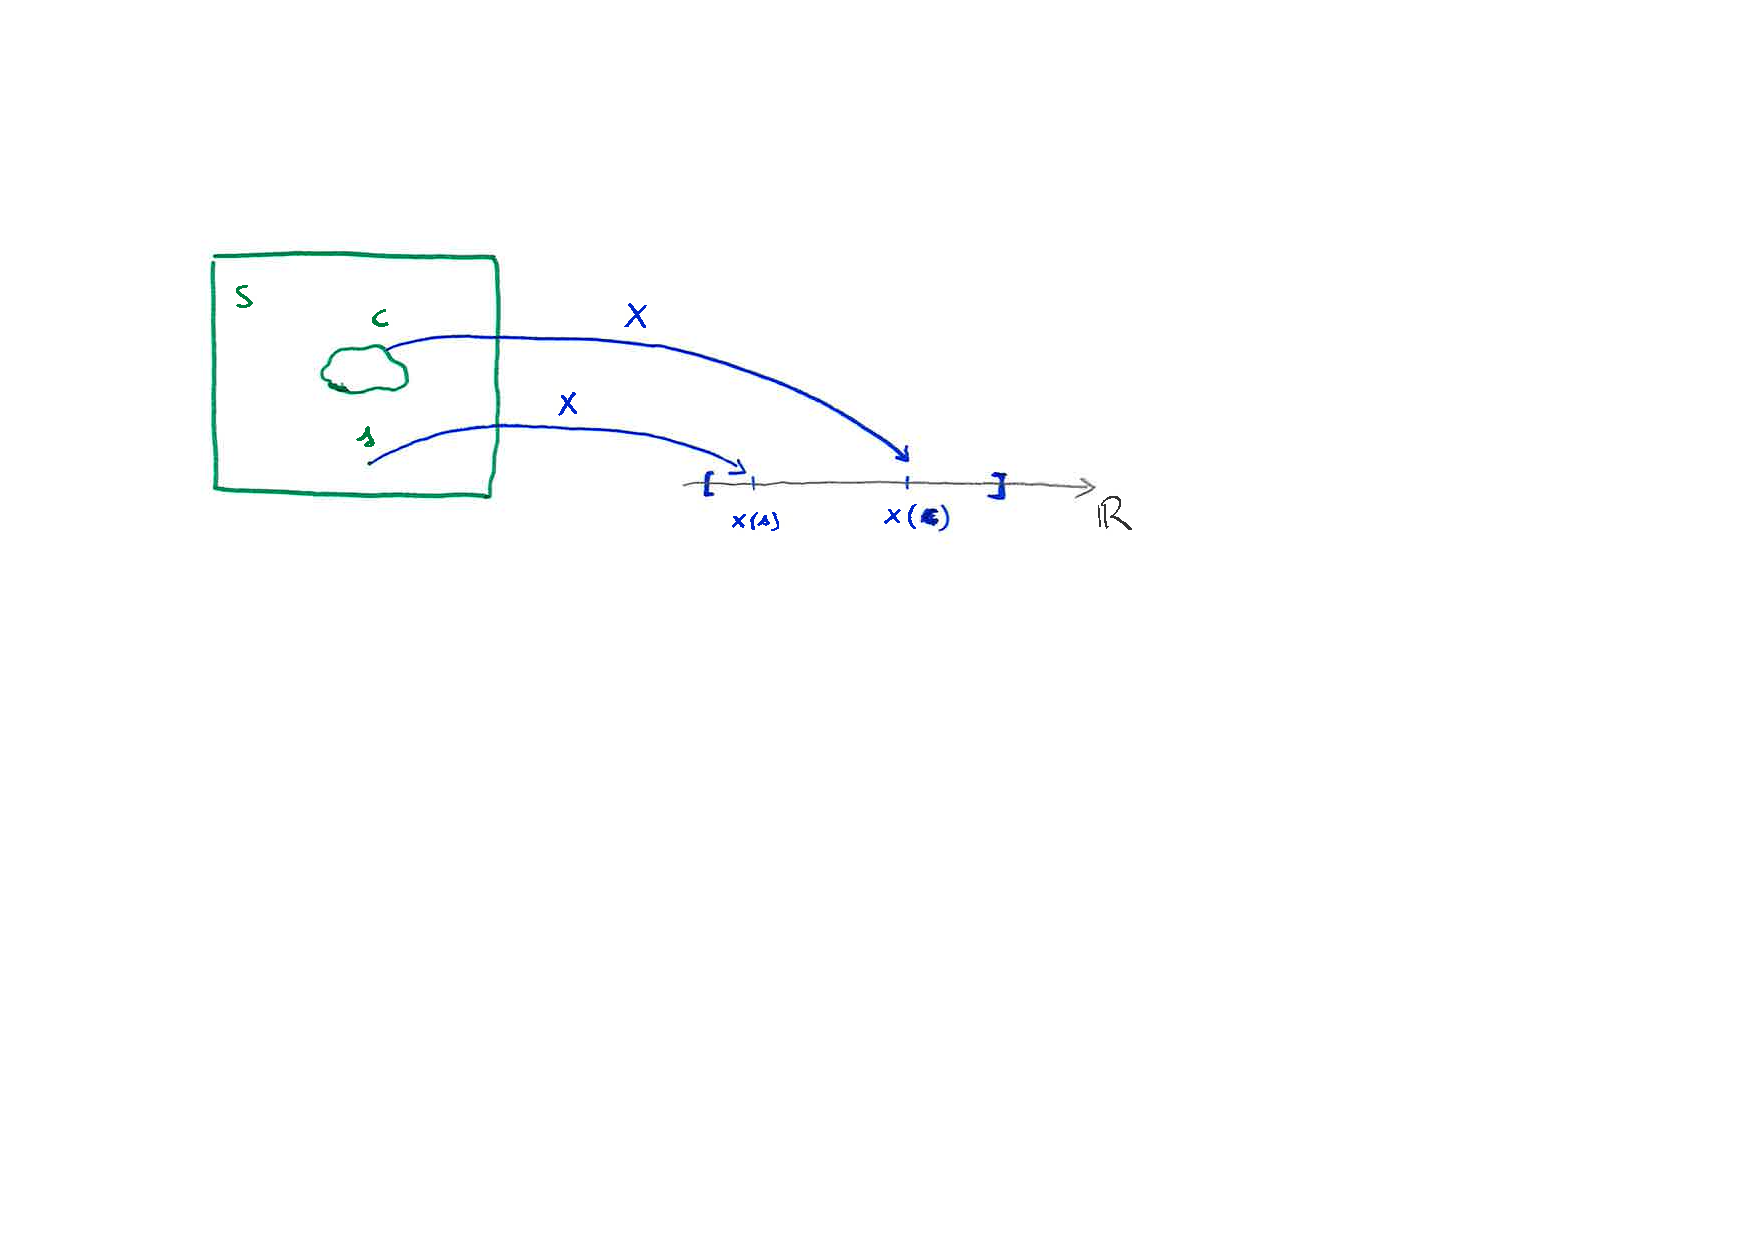
\includegraphics[width=0.85\textwidth, height=0.65\textheight]{img/scan2.pdf}
\end{figure}
\end{minipage}
\end{frame}





\begin{frame}
\frametitle{Example: from $S$ to $D$, via $X(\cdot)$}

\begin{example} [Roll the die]

\textbf{Experiment:} We roll two dice and we consider the number of points in the first die, and the number of points in the second die. We already know that the sample space $\color{Mygreen}S\color{black}$ is given by:

\begin{figure}[h]
\centering
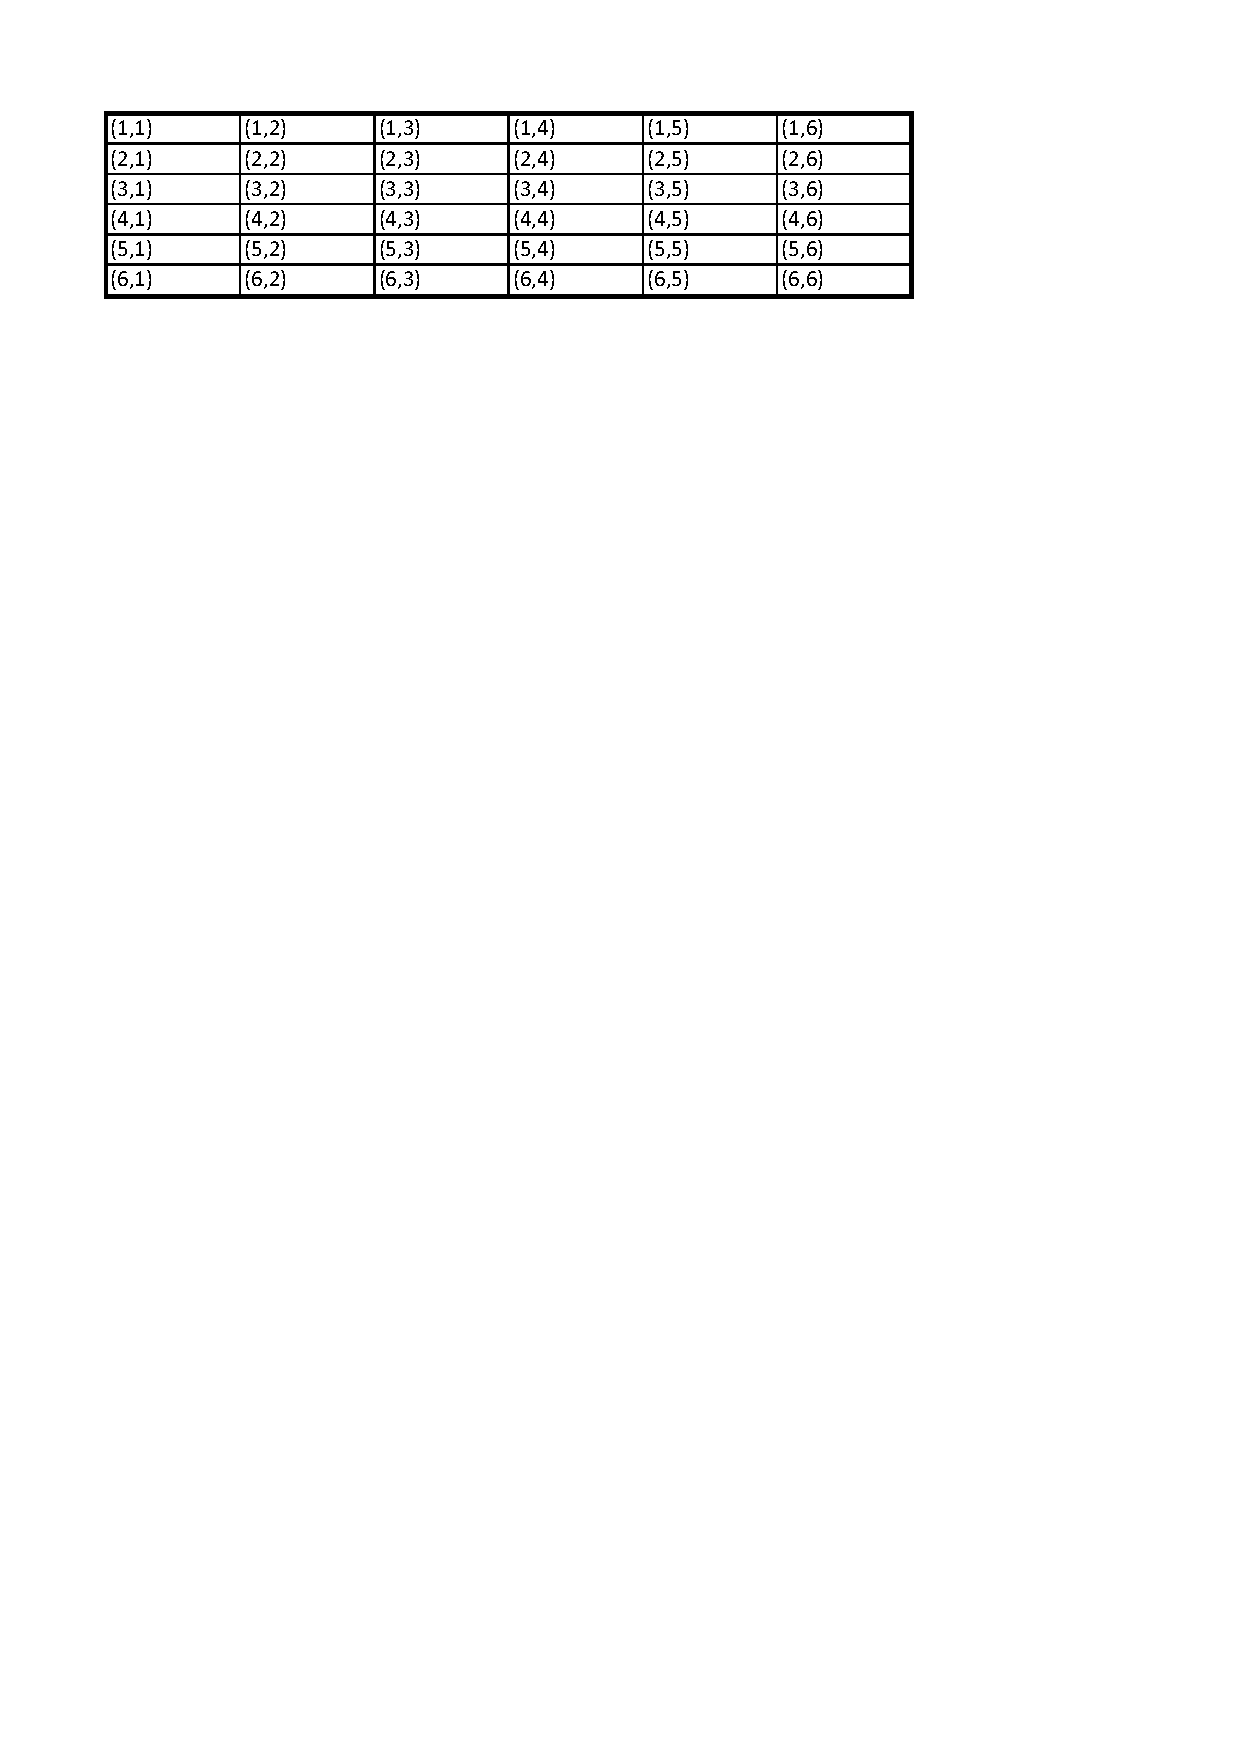
\includegraphics[width=0.8\textwidth,
height=0.3\textheight]{img/C.pdf}
\end{figure}
For the elements related to $\color{Mygreen}S\color{black}$ we have a probability $\color{Mygreen}Pr\color{black}$
%On $S$ we have the triplet $(S,\mathcal{B},Pr)$.
\end{example}

\end{frame}

\begin{frame}
\frametitle{From $S$ to $D$, via $X(\cdot)$}

\begin{example} [cont'd]
Now define $X(\color{Mygreen}s_{ij}\color{black})$ as the sum of the outcome of the outcome $i$ of the first die and the outcome $j$ of the second die. Thus:
\begin{eqnarray*}
X(\color{Mygreen}s_{ij}\color{black})= X(i,j)= i+j, & \textit{for} & i=1,...,6,  \textit{and  }   j=1,...,6
\end{eqnarray*}
%where $i$ is the outcome of the first die, while $j$ is the outcome of the second die.
In this notation $\color{Mygreen}s_{ij}\color{black}=(i,j)$ and $\color{Mygreen} s_{ij} \in S \color{black}$, each having probability $1/36$.\pause
\vspace{0.1cm}

\textbf{Facts:}
\begin{itemize}
\item $X(\cdot)$ maps $\color{Mygreen} S \color{black}$ into $\color{blue}D\color{black}$. \pause The (new) sample space $\color{blue}D\color{black}$ is given by
\begin{equation*}
\color{blue}D=\left\{2,3,4,5,6,7,8,9,10,11,12\right\}\color{black}
\end{equation*}
where, e.g., $\color{blue}2\color{black}$ is related to the pair $(1,1)$, $\color{blue}3\color{black}$ is related to the pairs $(1,2)$ and $(2,1)$, etc etc. To $\color{blue}D\color{black}$ is related the new $\color{blue}{P}\color{black}$
%triplet $(\color{blue}D\color{black},\mathcal{B}_{\color{blue}{D}\color{black}},P)$ .\pause


\end{itemize}
\end{example}
\end{frame}

\begin{frame}
\frametitle{From $S$ to $D$, via $X(\cdot)$}

\begin{example} [cont'd]

\begin{itemize}
\item To each element (event) in $\color{blue}D\color{black}$ we can attach a probability, using the probability of the corresponding event(s) in $S$. For instance,
$$
P(\color{blue}2\color{black})=Pr(1,1)=1/36, \quad \text{or} \quad P(\color{blue}3\color{black})=Pr(1,2)+Pr(2,1)=2/36.
$$
\vspace{-0.3cm}
\item How about the $P(\color{blue}7\color{black})$?
\begin{equation*}
P(\color{blue}7\color{black})=Pr(3,4)+Pr(2,5)+Pr(1,6)+Pr(4,3)+Pr(5,2)+Pr(6,1)=6/36.
\end{equation*}
\vspace{-0.3cm}
\item The latter equality can also be re-written as
\[P(\color{blue}7\color{black})=2(Pr(3,4)+Pr(2,5)+Pr(1,6))=6 \ Pr(3,4),\]
\vspace{-0.3cm}
\item What is $P(\color{blue} 9 \color{black})$? What is $P(\color{blue} 13 \color{black})$? [Hint: does \color{blue} 13 \color{black} belong to $\color{blue} D \color{black}$?]

\end{itemize}
\end{example}
\end{frame}





\begin{frame}%

\frametitle{Formal definition of a random variable (II)}
Let us formalize all these ideas:
\begin{stepitemize}
%\item $X$ is called a random variable if it satisfies the conditions stated below
\vspace{0.25cm}
\item Let $D$ be the set of all values $x$ that can be obtained by $X\left(
s\right) $, for all $s\in S$:%
\begin{equation*}
D=\left\{ x:x=X\left( s\right) ,\text{ }s\in S\right\}
\end{equation*}
%\vspace{0.5cm}
\item $D$ is a list of all possible numbers $x$ that can be obtained, and
thus is a \textbf{sample space }for\textbf{\ }$X$. \textit{Remark that the random variable is $X$
while $x$ represents its realization (non random).}
\vspace{0.25cm}
\item $D$ can be either an \textbf{uncountable interval} (then $X$ is a \textbf{%
continuous} random variable), or
\vspace{0.25cm}
\item $D$ can be \textbf{discrete} or \textbf{countable} (the $X$ is a
\textbf{discrete} random variable)
\end{stepitemize}

%TCIMACRO{\TeXButton{EndFrame}{\end{frame}}}%
%BeginExpansion
\end{frame}%
%EndExpansion

%%TCIMACRO{\TeXButton{BeginFrame}{\begin{frame}}}%
%%BeginExpansion
%\begin{frame}%
%%EndExpansion
%
%\frametitle{Formal definition of a random variable II}
%
%\begin{stepitemize}
%\item Let $D$ be the set of all values $x$ that can be obtained by $X\left(
%c\right) $, for all $c\in \mathcal{C}$:%
%\begin{equation*}
%D=\left\{ x:x=X\left( c\right) ,\text{ }c\in \mathcal{C}\right\}
%\end{equation*}
%
%\item $D$ is a list of all possible numbers $x$ that can be obtained, and
%thus is a \textbf{sample space }for\textbf{\ }$X$
%
%\item $D$ can be either an \textbf{interval} (then $X$ is a \textbf{%
%continuous} random variable), or
%
%\item $D$ can be \textbf{discrete} or \textbf{countable} (the $X$ is a
%\textbf{discrete} random variable)
%\end{stepitemize}
%
%%TCIMACRO{\TeXButton{EndFrame}{\end{frame}}}%
%%BeginExpansion
%\end{frame}%
%%EndExpansion

%TCIMACRO{\TeXButton{BeginFrame}{\begin{frame}}}%
%BeginExpansion
\begin{frame}%
%EndExpansion

\frametitle{Formal definition of a random variable (III)}

%\begin{stepitemize}
%\vspace{0.15cm}
%\item
For $X$ to be a random variable it is required that
%\vspace{0.15cm}
%\item the set
%\begin{equation*}
%\mathcal{B}_{d}=\left\{ s\in S:X\left( s\right) \leq d\right\}
%\end{equation*}%
%belongs to $\mathcal{B}$ for all $d\in D$
%\vspace{0.15cm}
%\item The $\sigma $-algebra $\mathcal{B}_{D}$ generated by $D$ is obtained
%by taking unions, intersections and complements of the sets $\mathcal{B}_{d}$
%\vspace{0.15cm}
%\item Then, for each $A\in \mathcal{B}_{D}$ we can define%
for each $A$ (as ``made'' by elements in $D$)
\begin{equation*}
\color{blue}P\color{black}\left( A\right) = \color{Mygreen} {Pr} \color{black}( \left\{ s\in S :X\left(  s  \right) \in
A\right\})
\end{equation*}
where $\color{blue}P \color{black}$ and $\color{Mygreen} Pr \color{black}$ stand for ``probability'' on $\color{blue} D \color{black}$
and on $\color{Mygreen} S \color{black}$, respectively.
%\end{stepitemize}
%TCIMACRO{\TeXButton{EndFrame}{\end{frame}}}%
%BeginExpansion
%\end{frame}%
%\begin{frame}%
%\frametitle{Formal definition of a random variable (III)}
%\begin{stepitemize}
%\item One can show that the assumptions of probability hold:
%\end{stepitemize}
%\vspace{0.5cm}
So
\begin{enumerate}

\item $P \left( A\right) \geq 0$ %for all $A\in \mathcal{B}_{D}$
\vspace{0.15cm}
\item $\color{blue}P \left( D\right) \color{black}=\color{Mygreen}Pr (\left\{ s\in S:X\left( s\right)
\in D\right\}) =Pr \left( S\right) =1 \color{black}$
\vspace{0.15cm}
\item If $A_{1},A_{2},A_{3}...$ is a sequence of events %sets in $\mathcal{B}_{D}$
such that $$A_{i}\cap A_{j}=\varnothing $$ for all $i\neq j$ then
$$\color{blue}P \color{black} \left(
\bigcup _{i=1}^{\infty }A_{i}\right) =\sum_{i=1}^{\infty } \color{blue} P  \color{black} \left(
A_{i}\right) . $$
\end{enumerate}
From now on, I drop the colors.
\end{frame}%



%\begin{frame}
%\frametitle{Formal definition of a random variable (graphical)}
%%Just for the sake of this picture, let us set
%%$$\Omega=S \quad s = \omega_i \quad D= \mathbb{R}.
%%$$
%%Then, we have the following graphical representation for a random variable:
%
%\begin{minipage}{1.0\textwidth}
%\begin{figure}[h!]
%\centering
%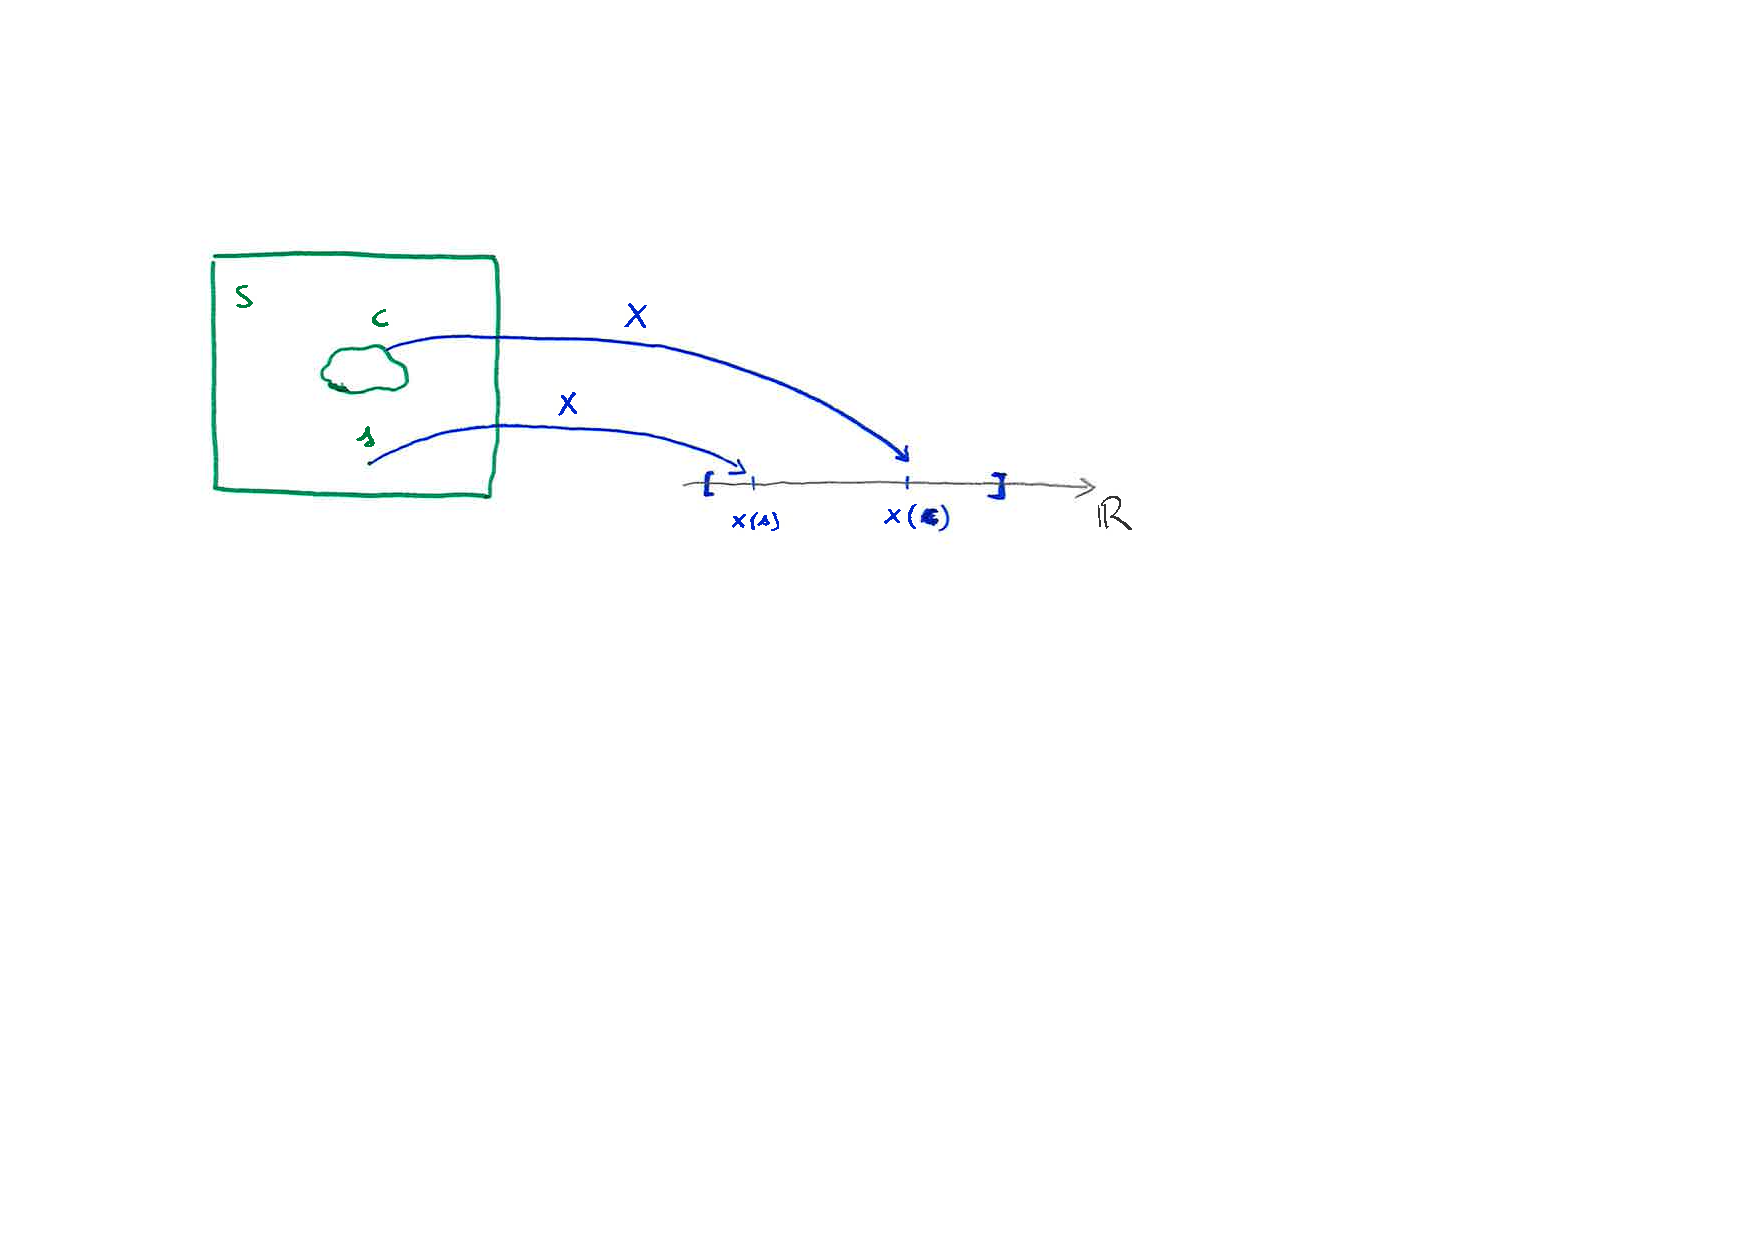
\includegraphics[width=0.85\textwidth, height=0.65\textheight]{img/scan2.pdf}
%\end{figure}
%\end{minipage}
%\end{frame}
%


\begin{frame}%

\frametitle{An Example from gambling}

\begin{example} [Geometric random variable]
Consider the problem of rolling a die until a 6 appears.
\begin{stepitemize}
\item Let $X$ denote the number of rolls required for the process to end

\item The possible values of $X$ are: $1, 2, 3,\ldots,n,\ldots$ ($\equiv
\mathbb{N}$).

\item $P(\{X=1\}) =\Pr (\text{'6' appears on the 1st roll})= \frac{1}{6}$

\item $P (\{X=2\})=\Pr \left( \text{no `}6\text{' on the 1st roll and `}6\text{%
' on the 2nd roll}\right) =\frac{5}{6}\cdot \frac{1}{6}=\frac{5}{36}$

\item $P(\{X=3\})=\Pr \left( \text{no `}6\text{' on either the 1st or 2nd
roll and '6' on the third roll}\right)$\newline
$=\frac{5}{6}\cdot \frac{5}{6}\cdot \frac{1}{6}=\frac{25}{216}$

\item $\ldots$ and so on $\ldots$

\item $P(\{X=n\})=\Pr( \text{no `}6\text{' on the first }$n-1$\text{ rolls
and '6' on the last roll})$ \newline
$=\left(\frac{5}{6}\right)^{n-1}\cdot \frac{1}{6}$

\item $\ldots$ and so on $\ldots$.
\end{stepitemize}


\end{example}
\end{frame}%
%EndExpansion

%TCIMACRO{\TeXButton{BeginFrame}{\begin{frame}}}%
%BeginExpansion
\begin{frame}%
%EndExpansion

\frametitle{An Example from gambling}

\begin{example} [cont'd]
\begin{stepitemize}
\item Rather than list the possible values of $X$ along with the associated
probabilities in a table, we can provide a formula that gives the required
probabilities.

\item The probability distribution of the random variable $X$
is given by
\begin{equation*}
P(\left\{ X=n \right\})=\left(\frac{5}{6}\right)^{n-1}\frac{1}{6}\quad\text{for}%
\quad n=1,2,\ldots
\end{equation*}

\item Note that (using properties of geometric series)
\begin{equation*}
\sum_{n=1}^\infty\left(\frac{5}{6}\right)^{n-1}\frac{1}{6}=1.
\end{equation*}
\end{stepitemize}

%TCIMACRO{\TeXButton{EndFrame}{\end{frame}}}%
%BeginExpansion
\end{example}
\end{frame}%
%EndExpansion

%%TCIMACRO{\TeXButton{BeginFrame}{\begin{frame}}}%
%%BeginExpansion
%\begin{frame}%
%%EndExpansion
%
%\frametitle{Example (continued)}
%
%\begin{stepitemize}
%\item The cumulative distribution function (CDF) of the random variable $X$
%is
%
%%\item
%%\begin{equation*}
%%\begin{tabular}{|c|c|}
%%\hline
%%$x_{i}$ & $\Pr \left( X\leq x_{i}\right) $ \\ \hline\hline
%%$1$ & $\frac{1}{6}$ \\ \hline
%%$2$ & $\frac{11}{36}$ \\ \hline
%%$3$ & $1$ \\ \hline
%%\end{tabular}%
%%\end{equation*}
%\begin{equation*}
%\Pr ( X\leq n)=\sum_{r=1}^n\left(\frac{5}{6}\right)^{r-1}\cdot \frac{1}{6}%
%\quad\text{for}\quad n=1,2,\ldots
%\end{equation*}
%
%\item The CDF also provides a formula from which everything about the
%probability distribution of the random variable $X$ can be derived.
%\end{stepitemize}
%
%%TCIMACRO{\TeXButton{EndFrame}{\end{frame}}}%
%%BeginExpansion
%\end{frame}%
%%EndExpansion

\subsection{Discrete random variables}

%TCIMACRO{\TeXButton{BeginFrame}{\begin{frame}}}%
%BeginExpansion
\begin{frame}%
%EndExpansion

\frametitle{Discrete random variables}

Discrete random variables are often associated with the process of counting (see previous
example). More generally,
\begin{definition}
Suppose $X$ can take the values $x_{1},x_{2},x_{3},\ldots ,x_{n}$. The probability of $x_{i}$ is
$$p_{i}= P(\left\{ X=x_i\right\})$$

and we must have $p_{1}+p_{2}+p_{3}+\cdots +p_{n}=1$ and all $p_{i}\geq 0$. These probabilities may be put in a table%
\begin{equation*}
\begin{tabular}{|c|c|}
\hline
$x_i $ & $P(\left\{ X=x_i\right\}) $ \\ \hline\hline
$x_{1}$ & $p_{1}$ \\ \hline
$x_{2}$ & $p_{2}$ \\ \hline
$x_{3}$ & $p_{3}$ \\ \hline
$\vdots $ & $\vdots $ \\ \hline
$x_{n}$ & $p_{n}$ \\ \hline\hline
Total & $1$ \\ \hline
\end{tabular}%
\end{equation*}
\end{definition}
\end{frame}%

\begin{frame}%
%EndExpansion

\frametitle{Discrete random variables}


For a \textbf{discrete random variable $X$}, any table listing all
possible nonzero probabilities provides the entire \textbf{probability
distribution}. The \textbf{probability mass function} $p(a)$ of $X$ is defined by
$$ p_a = p(a)= P(\{X=a \}),
$$
and this is positive for at most a countable number of values of $a$. For instance,
$p_{1} = P(\left\{ X=x_1\right\})$, $p_{2} = P(\left\{ X=x_2\right\})$, and so on.
That is, if $X$ must assume
one of the values $x_1,x_2,...$, then
\bea
 p(x_i) \geq 0 & \text{for \ \ } i=1,2,... \nn \\
 p(x) = 0 & \text{otherwise.}
\eea

Clearly, we must have
$$
\sum_{i=1}^{\infty} p(x_i) = 1.
$$

%The probabilities $p_{i}=P\left( X=x_{i}\right)$ may be given by an appropriate mathematical formula: i.e.
%$$
%p_{i}=P\left( X=x_{i}\right)=f(x_{i})
%$$
%for a suitably specified function $f(\cdot)$ --- see. e.g.,  the Geometric
%random variable.


\end{frame}%

\begin{frame}%

\frametitle{Cumulative Distribution Function (I)}

The \textbf{cumulative distribution function} (\textbf{CDF}) is a
table listing the values that $X$ can take, along with
$$
F_X(a) = P \left(\{ X\leq a\}\right)= \sum_{\text{all \ \ } x \leq a } p(x).
$$
If the random variable $X$ takes on values $x_{1},x_{2},x_{3},\ldots .,x_{n}$ \emph{listed in
increasing order } $
x_{1}<x_{2}<x_{3}<\cdots <x_{n}
$, the CDF is a step function, that it its value is constant in the intervals $(x_{i-1},x_i]$ and takes a step/jump of size $p_i$
at each $x_i$:
\vspace{0.1cm}

\begin{equation*}
\begin{tabular}{|c|c|}
\hline
$x_i $ & $F_X(x_i) =P \left(\{ X\leq x_i\}\right) $ \\ \hline\hline
$x_{1}$ & $p_{1}$ \\ \hline
$x_{2}$ & $p_{1}+p_{2}$ \\ \hline
$x_{3}$ & $p_{1}+p_{2}+p_{3}$ \\ \hline
$\vdots $ & $\vdots $ \\ \hline
$x_{n}$ & $p_{1}+p_{2}+\cdots +p_{n}=1$ \\ \hline
\end{tabular}%
\end{equation*}

\vspace{0.2cm}


%TCIMACRO{\TeXButton{EndFrame}{\end{frame}}}%
%BeginExpansion
\end{frame}%
%EndExpansion



\begin{frame}

\frametitle{Cumulative Distribution Function (II)}

\begin{example}

\noindent
\begin{center}
\begin{tabular}{c|cccc|c}
$x_i$ & 0 & 1 & 2 & 3 & Tot \\ \hline
$P(\{X=x_i\})$ & 4/35 & 18/35 & 12/35 & 1/35 & 1 \\
$P(\{X\leq x_i\})$ & 4/35 & 22/35 & 34/35 & 35/35 &
\end{tabular}
\end{center}

\bigskip
$$F_X(x) = \left\{
\begin{array}{ll}
0 & x<0 \\
4/35 & 0 \leq x < 1\\
22/35 & 1 \leq x < 2\\
34/35 & 2 \leq x < 3 \\
1 & x \geq 3.
\end{array} \right.$$

\end{example}

\end{frame}


\begin{frame}

\frametitle{Cumulative Distribution Function (III)}

\begin{example} [cont'd]

... or graphically, you get \textit{a step function} ...

\begin{figure}[h!]
\centering
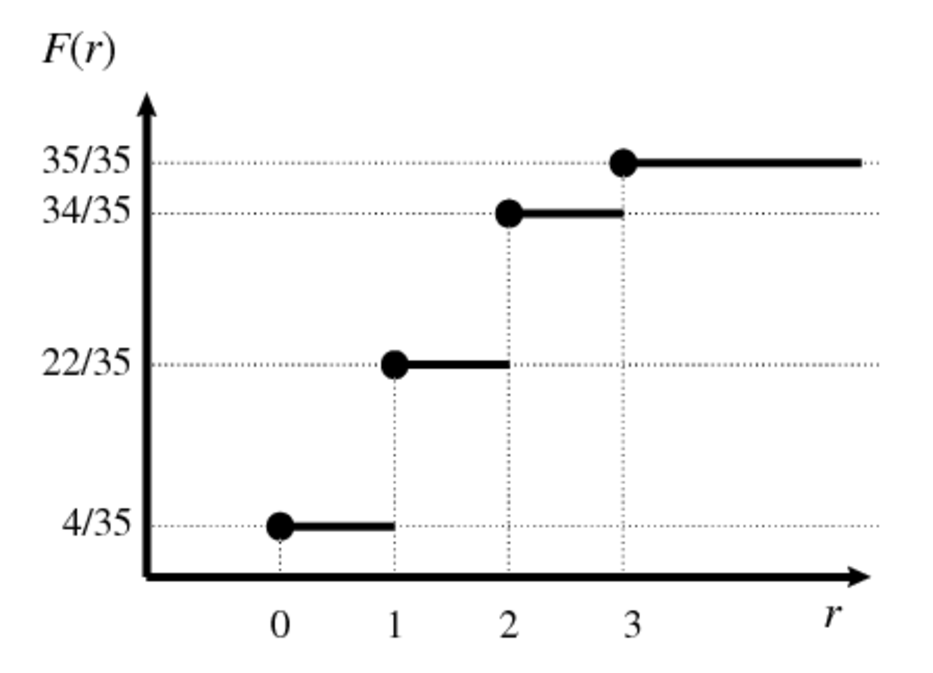
\includegraphics[width=0.5\textwidth,height=0.5\textheight]{img/repartbis.pdf}
\end{figure}

\end{example}


\end{frame}



\begin{frame}

\frametitle{Cumulative Distribution Function (IV)}

\begin{remark}
Suppose $a\leq b$. Then, because the event $\{X\leq a \}$ is contained in the event $\{X\leq b \}$, namely
$$
\{X\leq a \} \subseteq \{X\leq b \},
$$
 it follows that
 $$F_X(a) \leq F_X(b),
 $$
so, the probability of the former is less than or equal to the probability of the latter. \\
\vspace{0.5cm}
\begin{center}
\textbf{In other words, $F_X(x)$ is a nondecreasing function of $x$.}
\end{center}
\end{remark}


\end{frame}



\begin{frame}

\frametitle{Cumulative Distribution Function (V)}

\begin{example} [Quantiles]

The CDF can be inverted to define the value $x$ of $X$ that corresponds to a given probability $\alpha$, namely $\alpha = P (X \leq x )$, for $\alpha \in [0,1]$. \\ \vspace{0.4cm}


The inverse CDF $F_X^{-1}(\alpha)$ or quantile of order $\alpha$, and labelled as  $Q(\alpha)$, is the smallest
realisation of $X$ associated to a CDF greater or equal to $\alpha$; in formula, the
$\alpha$-quantile $Q(\alpha)$ is the smallest number satisfying:

$$
F_X [F^{-1}_X (\alpha)] = P[X \leq \underbrace{F^{-1}_X (\alpha)}_{Q(\alpha)}] \geq \alpha, \quad \text{for} \quad \alpha\in[0,1].
$$

By construction, a quantile of a discrete random variable is a realization of $X$. More to come in Lecture 5...

\end{example}


\end{frame}

\begin{frame}

\frametitle{Cumulative Distribution Function (VI)}

\begin{example} [cont'd, graphically]


\begin{figure}[h!]
\centering
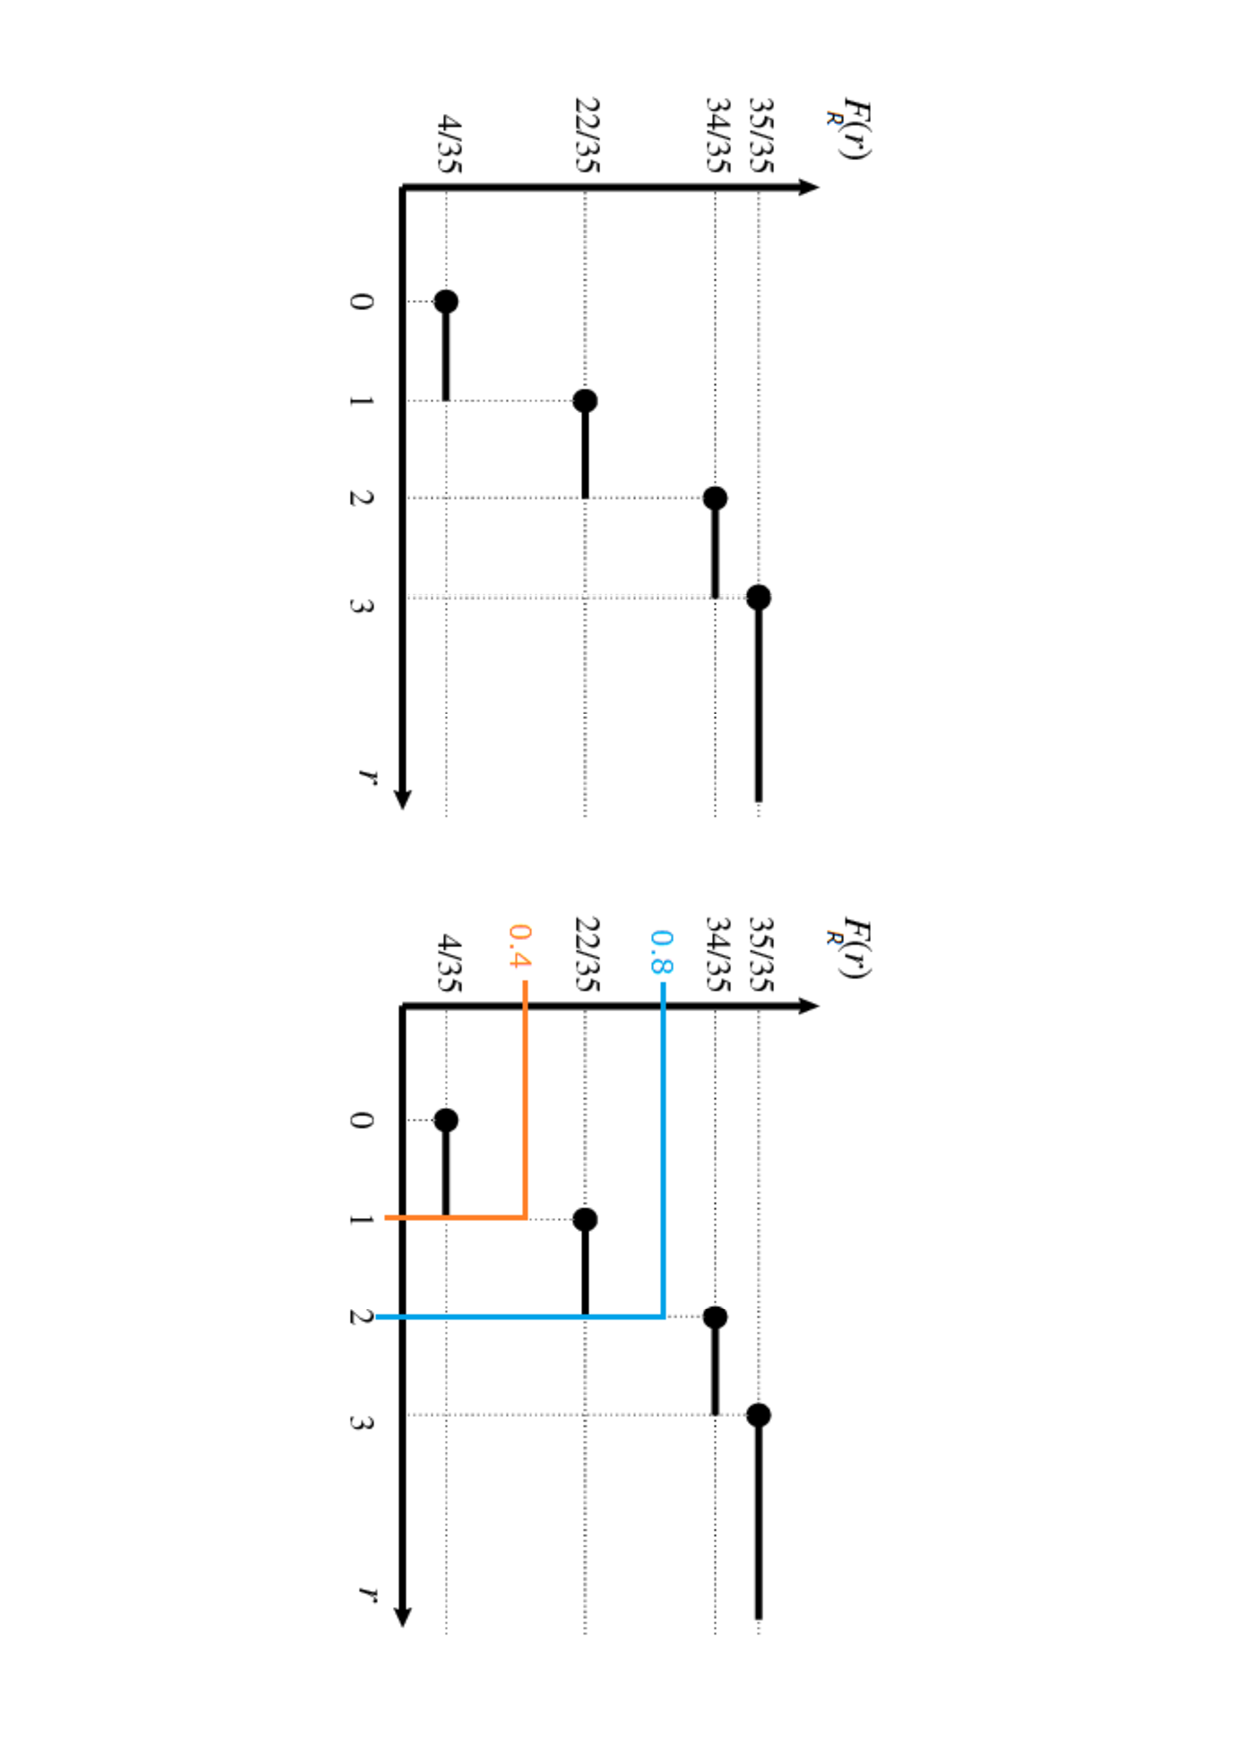
\includegraphics[width=0.5\textwidth,height=0.95\textheight, angle = 90]{img/Quantiles_Discr.pdf}
\end{figure}
...calling (only for this slide) $R$ the rv, $r$ its realizations and $F_R(r)$ its CDF at $r$...
\end{example}


\end{frame}



%TCIMACRO{\TeXButton{BeginFrame}{\begin{frame}}}%
%BeginExpansion
\begin{frame}%
%EndExpansion

\frametitle{Distributional summaries for discrete random variables}

\begin{stepitemize}
\item For a discrete random variable, it is useful to describe some
attributes or properties of the distribution

\begin{stepitemize}
\item such as a measure of location and a measure of spread
\end{stepitemize}

\item The \textbf{expected value}, or\textbf{\ mean value}, of the
distribution \begin{equation*}
E\left[ X\right] =p_{1}x_{1}+p_{2}x_{2}+\cdots + p_{n}x_{n} = \sum_{i=1}^{n} p_i x_i
\end{equation*}%
is a measure of \emph{location} --- roughly speaking this is the \emph{center} of the distribution;


\item The \textbf{square root of the variance}, or\textbf{\ standard
deviation,} of the distribution%
\begin{eqnarray*}
s.d\left( X\right) &=&\sqrt{Var\left( X\right) } \\
&=&\sqrt{p_{1}\left( x_{1}-E\left[ X\right] \right) ^{2}+p_{2}\left( x_{2}-E%
\left[ X\right] \right) ^{2}+\cdots + p_{n}\left( x_{n}-E\left[ X\right]
\right) ^{2}}
\end{eqnarray*}%
is a measure of \emph{spread (or `variability' or `dispersion').}
\end{stepitemize}

%TCIMACRO{\TeXButton{EndFrame}{\end{frame}}}%
%BeginExpansion
\end{frame}%
%EndExpansion

%TCIMACRO{\TeXButton{BeginFrame}{\begin{frame}}}%
%BeginExpansion
\begin{frame}%
%EndExpansion

\frametitle{Important properties}

If $X$ is a discrete random variable and $a$ is any real number, then

\vspace{0.2cm}

\begin{stepenumerate}
\item $E\left[ \alpha X\right] =\alpha E\left[ X\right] $

\item $E\left[ \alpha+X\right] =\alpha+E\left[ X\right] $

\item $Var\left( \alpha X\right) =\alpha^{2}Var\left( X\right) $

\item $Var\left( \alpha+X\right) =Var\left( X\right) $
\end{stepenumerate}

\begin{exercise}
Let us very the first property:
$
E\left[ \alpha X \right] =\alpha E\left[ X\right].
$
From the Intro lecture we know that, for every $\alpha_i \in \mathbb{R}$,
$$\sum_{i=1}^{n} \alpha_i X_{i} = \alpha_1 X_1 + \alpha_2 X_2 +....+ \alpha_n X_n.$$ So, the
required result follows as a special case, setting $\alpha_i= \alpha$, for every $i$, and applying the definition
of expected value. Verify this and the other properties as an exercise. [Hint: set $\alpha_i = \alpha p_i$.]
\end{exercise}

\end{frame}

\begin{frame}

\frametitle{Dependence/Independence}

\begin{definition}
Consider two discrete random variables\footnote{Technically speaking, $X$ and $Y$ should be defined on the same probability space,
%$(S,\mathcal{B},P)$,
but we do not pursue this argument.} $X$ and $Y$. Then, $X$ and $Y$ are \textbf{independent} if%
\begin{equation*}
P \left(\left\{ \ X=x\right\} \cap \left\{ Y=y\right\} \right) =P \left(\{
X=x\}\right) \cdot P \left(\{ Y=y \}\right)
\end{equation*}
for all values $x$ that $X$ can take and all values $y$ that $Y$ can take.
\end{definition}

\end{frame}%
%EndExpansion

%TCIMACRO{\TeXButton{BeginFrame}{\begin{frame}}}%
%BeginExpansion
\begin{frame}%
%EndExpansion

\frametitle{More important properties}

\begin{stepitemize}
\item If $X$ and $Y$ are two discrete random variables, then%
\begin{equation*}
E\left[ X+Y\right] =E\left[ X\right] +E\left[ Y\right]
\end{equation*}

\item If $X$ and $Y$ are also \emph{independent}, then%
\begin{equation}
Var\left( X+Y\right) =Var\left( X\right) +Var\left( Y\right) \label{Eq. Var}
\end{equation}

\begin{remark}
Note that Eq. (\ref{Eq. Var})  does not (typically) hold if $X$ and $Y$ are NOT independent---more to come on this later on...
\end{remark}
\end{stepitemize}

%TCIMACRO{\TeXButton{EndFrame}{\end{frame}}}%
%BeginExpansion
\end{frame}%
%EndExpansion

%TCIMACRO{\TeXButton{BeginFrame}{\begin{frame}}}%
%BeginExpansion
\begin{frame}%
%EndExpansion

\frametitle{More on expectations}

Recall that the expectation of X was defined as
\begin{equation*}
E\left[ X\right] = \sum_{i=1}^{n} p_i x_i
\end{equation*}

Now, suppose we are interested in a function $m$ of the random variable $X$, say $m(X)$. We define
\begin{equation*}
E\left[ m\left( X\right) \right] =p_{1}m\left( x_{1}\right) +p_{2}m\left(
x_{2}\right) +\cdots p_{n}m\left( x_{n}\right).
\end{equation*}

Notice that the variance is a special case of expectation where,
\begin{equation*}
m(X)=(X-E\left[ X\right] )^{2}.
\end{equation*}
Indeed,
\begin{equation*}
Var\left( X\right) =E\left[ (X-E\left[ X\right] )^{2}\right].
\end{equation*}

\begin{exercise}
Show that
\begin{equation*}
Var\left( X\right) =E\left[ X^{2}\right] -E\left[ X\right] ^{2}.
\end{equation*}
\end{exercise}

\end{frame}


%TCIMACRO{\TeXButton{BeginFrame}{\begin{frame}}}%
%BeginExpansion
\begin{frame}%
%EndExpansion

\frametitle{Some discrete distributions of interest}

\begin{stepitemize}
\item Discrete Uniform
\vspace{0.15cm}
\item Bernoulli
\vspace{0.15cm}
\item Binomial
\vspace{0.15cm}
\item Poisson
\vspace{0.15cm}
\item Hypergeometric
\vspace{0.15cm}
\item Negative binomial
\end{stepitemize}

\vspace{0.5cm}
Their main characteristic is that the probability $P\left(\left\{ X=x_i\right\}\right)$ is given by an appropriate mathematical formula: i.e.
$$
p_{i}=P\left(\left\{ X=x_i\right\}\right)=h(x_{i})
$$
for a suitably specified function $h(\cdot)$.

%TCIMACRO{\TeXButton{EndFrame}{\end{frame}}}%
%BeginExpansion
\end{frame}%
%EndExpansion

%TCIMACRO{\TeXButton{BeginFrame}{\begin{frame}}}%
%BeginExpansion
\begin{frame}%
%EndExpansion

\frametitle{Discrete uniform distribution}
\begin{small}
\begin{definition}
We say $X$ has a \textbf{discrete uniform distribution} when

\begin{stepitemize}
\item $X$ can take the values $x=0,1,2,...,k$ (for some specified finite value $k\in \mathbb{N}$)

\item The probability that $X=x$ is $1/\left( k+1\right) $, namely
$$
P\left(\left\{ X=x\right\}\right) = \frac{1}{\left( k+1\right)}.
$$
\end{stepitemize}

The probability distribution is given by
\begin{small}
\begin{equation*}
\begin{tabular}{|c|c|}
\hline
$x_i$ & $P \left(\left\{ X=x_i\right\}\right) $ \\ \hline\hline
$0$ & $\frac{1}{\left( k+1\right) }$ \\ \hline
$1$ & $\frac{1}{\left( k+1\right) }$ \\ \hline
$\vdots $ & $\vdots $ \\ \hline
$k$ & $\frac{1}{\left( k+1\right) }$ \\ \hline\hline
Total & $1$ \\ \hline
\end{tabular}%
\end{equation*}
\end{small}
\end{definition}
\end{small}
\end{frame}

\begin{frame}

\frametitle{Discrete uniform: expected value}

\begin{stepitemize}
\item The expected value of $X$ is%
\begin{eqnarray*}
E\left[ X\right] &=&  x_1 p_1 + ... +  x_k p_k\\
&=& 0\cdot \frac{1}{\left( k+1\right) }+1\cdot \frac{1}{%
\left( k+1\right) }+\cdots +k\cdot \frac{1}{\left( k+1\right) } \\
&=&\frac{1}{\left( k+1\right) }\cdot\left( 0+1+\cdots +k\right) \\
&=&\frac{1}{\left( k+1\right) }\cdot \frac{k\left( k+1\right) }{2} \\
&=&\frac{k}{2}.
\end{eqnarray*}

E.g. when $k=6$, then $X$ can take on one of the seven distinct values
$x=0,1,2,3,4,5,6,$ each with equal probability $\frac{1}{7}$, but the
expected value of $X$ is equal to $3$, which is  one of the possible outcomes!!!

\end{stepitemize}

%TCIMACRO{\TeXButton{EndFrame}{\end{frame}}}%
%BeginExpansion
\end{frame}%
%EndExpansion

%TCIMACRO{\TeXButton{BeginFrame}{\begin{frame}}}%
%BeginExpansion
\begin{frame}%
%EndExpansion

\frametitle{Discrete uniform: variance}

\begin{stepitemize}
\item The variance of $X$ -- we will be denoting it as $Var(X)$  -- is%
\begin{eqnarray*}
Var\left( X\right) &=&\left( 0-\frac{k}{2}\right) ^{2}\cdot \frac{1}{\left(
k+1\right) }+\left( 1-\frac{k}{2}\right) ^{2}\cdot \frac{1}{\left(
k+1\right) }+ \\
&&\cdots +\left( k-\frac{k}{2}\right) ^{2}\cdot \frac{1}{\left( k+1\right) }
\\
&=&\frac{1}{\left( k+1\right) }\cdot\left\{ \left( 0-\frac{k}{2}\right)
^{2}+\left( 1-\frac{k}{2}\right) ^{2}+\cdots +\left( k-\frac{k}{2}\right)
^{2}\right\} \\
&=&\frac{1}{\left( k+1\right) }\cdot \frac{k\left( k+1\right) \left(
k+2\right) }{12} \\
&=&\frac{k\left( k+2\right) }{12}
\end{eqnarray*}

E.g. when $k=6$, the variance of $X$ is equal to $4,$ and the standard
deviation of $X$ is equal to $\sqrt{4}=2.$
\end{stepitemize}

\end{frame}%

\begin{frame}%
\frametitle{Some illustrations of discrete uniform}

\begin{figure}[ptb]\centering
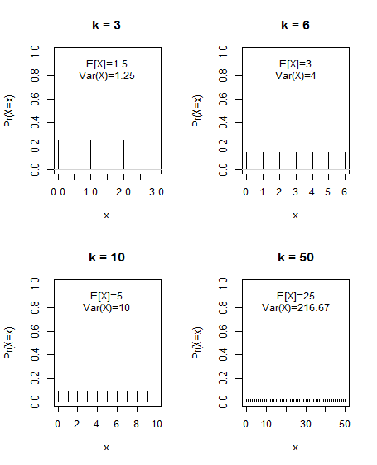
\includegraphics[width=0.55\textwidth, height=0.8 \textheight]{img/discrete_uniforms__1.pdf}%
\end{figure}
\end{frame}

\begin{frame}%
\frametitle{Some illustrations of discrete uniform}

\begin{example}

An example of discrete uniform is related to the experiment of rolling a die---remark, the outcome zero is not allowed in this specific example. \\ \vspace{0.3cm}

Let us call $X$ the corresponding random variable and $\{x_1,x_2,...,x_6\}$ its realizations.  \\ \vspace{0.3cm}

The possible outcomes
are
$$
\{1,2,3,4,5,6\}
$$
each having probability $\frac{1}{6}$. \vspace{0.3cm}

Moreover,

$$
E(X) = (1+2+3+4+5+6) \cdot \frac{1}{6} = 3.5,
$$

which is not one of the possible outcomes!!!

\end{example}

\end{frame}

\begin{frame}%
\frametitle{Bernoulli Trials}
\begin{definition}

\textit{Bernoulli trial} is the name given to the random variable $X$ having probability distribution given by%

\begin{equation*}
\begin{tabular}{|l|l|}
\hline
$x_i$ & $P(\left\{ X=x_i\right\}) $ \\ \hline\hline
$1$ & $p$ \\ \hline
$0$ & $1-p$ \\ \hline
\end{tabular}%
\end{equation*}
\end{definition}

\vspace{0.5cm}

Often we write%
\begin{equation*}
P(\left\{ X=x\right\} ) =p^{x}\left( 1-p\right) ^{1-x}, \quad \text{ for }x=0,1
\end{equation*}

%TCIMACRO{\TeXButton{EndFrame}{\end{frame}}}%
%BeginExpansion
\end{frame}%


\begin{frame}%
\frametitle{Bernoulli Trials}

A Bernoulli trial represents the most primitive form of all random variables. It derives from a random experiment having only two possible mutually exclusive outcomes. These are often labelled Success and Failure and

%\vspace{0.5cm}

\begin{stepitemize}
\item Success occurs with probability $p$
%\vspace{0.25cm}
\item Failure occurs with probability $1-p$.
\end{stepitemize}


%\vspace{0.5cm}
\begin{remark}
Just for the sake of notation, let us set $X=1$ if \emph{Success} occurs, and $X=0$ if \emph{Failure} occurs
\end{remark}


\begin{example}
Coin tossing:  we can define a random variable

\begin{equation*}
\begin{tabular}{|l|l|}
\hline
$x_i$ & $P(\left\{ X=x_i\right\}) $ \\ \hline\hline
$1$ & $p$ \\ \hline
$0$ & $1-p$ \\ \hline
\end{tabular}%
\end{equation*}
and say that $X=1$ if $H$ and $X=0$ if $T$.

\end{example}

\end{frame}

\begin{frame}%
%EndExpansion

\frametitle{Bernoulli Trials}

\begin{stepitemize}
\item Mean:
\begin{eqnarray*}
E\left[ X\right] &=&1 \cdot p+0 \cdot (1-p) \\
&=&p
\end{eqnarray*}

\item Variance:%
\begin{eqnarray*}
Var\left( X\right) &=&\left( 1-p\right) ^{2} \cdot p+\left( 0-p\right)
^{2} \cdot \left( 1-p\right) \\
&=&p\left( 1-p\right).
\end{eqnarray*}
\end{stepitemize}




\end{frame}%

\begin{frame}%

\frametitle{The Binomial Distribution}

\begin{definition}
Let us consider the  random experiment consisting in a series of $n$ trials having 3
characteristics

\begin{stepenumerate}
\item Only two mutually exclusive outcomes are possible in each trial: \emph{%
success} (\emph{S}) and \emph{failure} (\emph{F})

\item The outcomes in the series of $n$ trials constitute independent events

\item The probability of success $p$ in each trial is constant from trial to
trial
\end{stepenumerate}

$X$ is the \emph{number of successes} occurring in $n$ (Bernoulli) trials. Binomial probability distribution given by%
\begin{eqnarray}
P ( \left\{ X=x\right\})  &=&\left(
\begin{array}{c}
n \nonumber \\
x%
\end{array}%
\right) p^{x}\left( 1-p\right) ^{n-x} \\
&=&\frac{n!}{x!\left( n-x\right) !}p^{x}\left( 1-p\right) ^{n-x},\text{ for }%
x=0,1,2,...,n \label{Eq: Binom}
\end{eqnarray}
\end{definition}

\end{frame}%


\begin{frame}%

\frametitle{The Binomial Distribution}

Recall (see Intro lecture) that combinations are defined as:

\begin{equation*}
\left(
\begin{array}{c}
n \\
k%
\end{array}%
\right) =\frac{n!}{k!\left( n-k\right) !}=C^{k}_{n}
\end{equation*}
and, for $n \geq k$, we say ``$n$ choose $k$''. \\
\vspace{0.4cm}
The binomial coefficient $\left(
\begin{array}{c}
n \\
k%
\end{array}%
\right)$
represents the number of possible combinations of $n$ objects taken $k$ at a time, without regard of the order. \\% Rozanov page 7
\vspace{0.4cm}
\color{blue} Thus, $C^{k}_{n}$ represents the number of different groups of size $k$ that could be selected from a set of $n$ objects
when the order of selection is not relevant. \color{black}

\end{frame}%

\begin{frame}
\frametitle{The Binomial Distribution}

So, ''What is the interpretation of the formula? "


\begin{stepenumerate}
\item The first factor $$\left(
\begin{array}{c}
n \\
x%
\end{array}%
\right) =\frac{n!}{x!\left( n-x\right) !}$$ is the number of different
combinations of individual `successes' and `failures'  in $n$ (Bernoulli) trials that result in a sequence containing a total of $%
x $ `successes' and $n-x$ `failures'.


\item The second factor $$p^{x}\left( 1-p\right) ^{n-x}$$ is the probability associated with any one
sequence of $x$ `successes' and $(n-x)$ `failures'.
\end{stepenumerate}

\begin{remark}
Short-hand notation: $$ X \sim \text{B}(x,n,p)$$
 or, occasionally, simply $ X \sim \text{B} (n,p)$ (no $x$ in the formula).
\end{remark}

\end{frame}%



\begin{frame}%

\frametitle{The Binomial Distribution: expectation and variance}

\begin{stepitemize}
\item Mean:
\begin{eqnarray*}
E\left[ X\right] &=&\sum_{x=0}^{n}x\Pr \left\{ X=x\right\} \\
&=&\sum_{x=0}^{n}x\left(
\begin{array}{c}
n \\
x%
\end{array}%
\right) p^{x}\left( 1-p\right) ^{n-x} = np
\end{eqnarray*}

%\begin{stepitemize}
%\item Here $\sum_{x=1}^{n}$ denotes the sum over each value of $x$ from $0$
%to $n$
%\end{stepitemize}
\item Variance:%
\begin{eqnarray*}
Var\left( X\right) &=&\sum_{x=0}^{n}\left( x-np\right) ^{2} P (\left\{
X=x\right\}) \\
&=&np\left( 1-p\right)
\end{eqnarray*}
\end{stepitemize}
\begin{remark}
Looking at (\ref{Eq: Binom}), we remark that the Bernoulli distribution is a special case ($n=1$)
of the Binomial distribution. Roughly speaking, ``a Binomial random variable arises when we sum $n$ independent
Bernoulli trails.''
\end{remark}
%TCIMACRO{\TeXButton{EndFrame}{\end{frame}}}%
%BeginExpansion
\end{frame}%
%EndExpansion

%TCIMACRO{\TeXButton{BeginFrame}{\begin{frame}}}%
%BeginExpansion



%\begin{frame}%
%%EndExpansion
%
%\frametitle{Some illustrations of Binomial \begin{small}(introducing a tool)\end{small}}
%Let us provide a graphical illustration of $X\sim B(x,n,p)$ via some numerical method. Specifically, we first  \color{blue}simulate \color{black} a large number of
%realizations of $X$, then we draw their \color{blue}histrogram \color{black} (or barplot). \\
%\vspace{0.3cm}
%%\begin{remark}
%A \textbf{histogram} is a representation of a distribution by means of rectangles whose widths represent class intervals and whose areas are proportional
%to the corresponding frequencies. The purpose of a histogram is to graphically summarize the distribution of a data set -- roughly speaking, a histogram is a graphical representation of a table of frequencies. \\
%\vspace{0.3cm}
%
%\begin{remark}[How to draw it?]
%The most common form of
%the histogram is obtained by splitting the range of the data into equal-sized bins. Then for each bin, the number of points from the data set
%that fall into each bin are counted. That is: on the \color{blue} vertical axis we read the (relative) frequency \color{black} (i.e., counts for each bin); on the \color{red} horizontal axis we read the observed values of $X$\color{black}. The classes can either be defined arbitrarily by the user or via some systematic rule.
%\end{remark}
%\end{frame}


\begin{frame}%
%EndExpansion

\frametitle{Some illustrations of Binomial}

... same barplot as in slide 30, just a bit fancier...

\begin{figure}[ptb]\centering
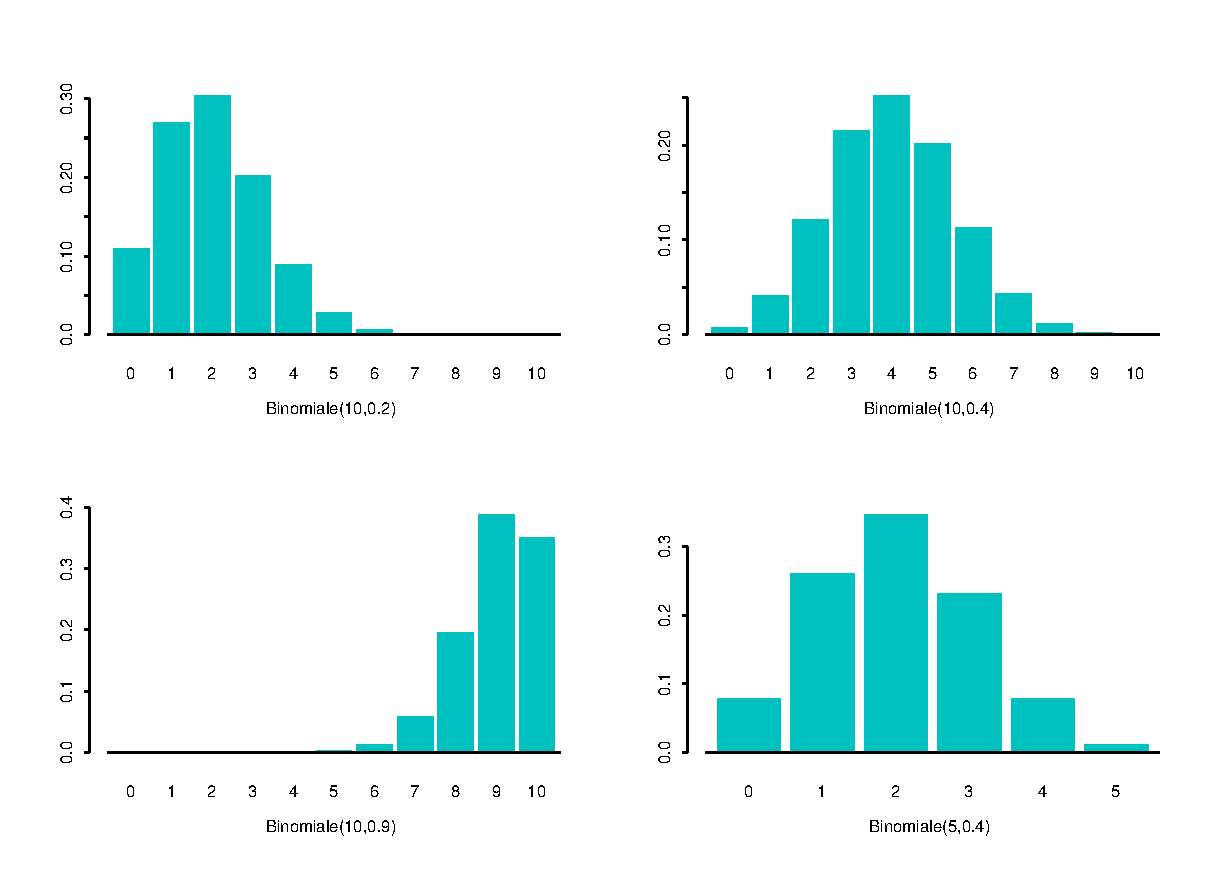
\includegraphics[width=0.75\textwidth,height=0.6\textheight]{img/distbin.pdf}
\end{figure}
\end{frame}%

\begin{frame}%
%EndExpansion


\frametitle{Binomial Distribution}

\begin{example} [cherry trees]

One night a storm washes three cherries ashore on an island. For each cherry, there is a probability $p=0.8$ that its seed will
produce a tree. What is the probability that these three cherries will produce two
trees?

\bigskip

First,  we notice that this can be determined using a \textbf{Bernoulli distribution}. To this end, consider whether each seed will produce a tree as a sequence of $n=3$
trials. For each cherry:

\begin{itemize}

\item either the cherry produces a tree (Success) or it
does not (Failure);
\item the event that a cherry produces a tree is independent from the event
that any of the other two cherries produces a tree.

\item The probability that a cherry produces a tree is the same for all
three cherries
\end{itemize}

\end{example}

\end{frame}%


\begin{frame}%

\frametitle{Binomial Distribution }

\begin{example} [cont'd]

\begin{figure}[ptb]\centering
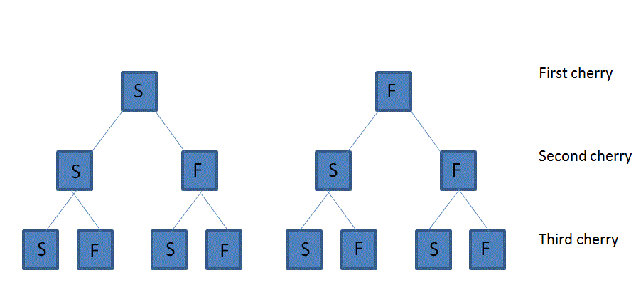
\includegraphics[]{img/BINOMIALpic__1.pdf}
\end{figure}

\end{example}
\end{frame}%

\begin{frame}%

\frametitle{Binomial Distribution}

\begin{example} [cont'd]

\begin{stepitemize}
\item There are $2^{3}=8$ possible outcomes from the $3$ individual trials

\item It does not matter which of the three cherries produce a tree

\item Consider all of the possible sequences of outcomes (S=success,
F=failure)%
\begin{equation*}
\text{SSS,
\color{red}%
SSF,
\color{black}%
\color{red}%
SFS%
\color{black}%
, SFF,
\color{red}%
FSS
\color{black}, FSF, FFS, FFF}
\end{equation*}

\item We are interested in
%TCIMACRO{\TeXButton{red}{\color{red}}}%
%BeginExpansion
\color{red}%
SSF%
%TCIMACRO{\TeXButton{black}{\color{black}}}%
%BeginExpansion
\color{black}%
,
\color{red}%
SFS%
%TCIMACRO{\TeXButton{black}{\color{black}}}%
%BeginExpansion
\color{black}%
%EndExpansion
,
%TCIMACRO{\TeXButton{red}{\color{red}}}%
%BeginExpansion
\color{red}%
%EndExpansion
FSS%
%TCIMACRO{\TeXButton{black}{\color{black}}}%
%BeginExpansion
\color{black}%
%EndExpansion

\item These possible events are \emph{mutually exclusive}, so%
\begin{equation*}
\Pr (\left\{
%TCIMACRO{\TeXButton{red}{\color{red}}}%
%BeginExpansion
\color{red}%
%EndExpansion
SSF%
%TCIMACRO{\TeXButton{black}{\color{black}}}%
%BeginExpansion
\color{black}%
%EndExpansion
\cup
%TCIMACRO{\TeXButton{red}{\color{red}}}%
%BeginExpansion
\color{red}%
%EndExpansion
SFS%
%TCIMACRO{\TeXButton{black}{\color{black}}}%
%BeginExpansion
\color{black}%
%EndExpansion
\cup
%TCIMACRO{\TeXButton{red}{\color{red}}}%
%BeginExpansion
\color{red}%
%EndExpansion
FSS%
%TCIMACRO{\TeXButton{black}{\color{black}}}%
%BeginExpansion
\color{black}%
%EndExpansion
\right\}) =\Pr (\left\{
%TCIMACRO{\TeXButton{red}{\color{red}}}%
%BeginExpansion
\color{red}%
%EndExpansion
SSF%
%TCIMACRO{\TeXButton{black}{\color{black}}}%
%BeginExpansion
\color{black}%
%EndExpansion
\right\}) +\Pr (\left\{
%TCIMACRO{\TeXButton{red}{\color{red}}}%
%BeginExpansion
\color{red}%
%EndExpansion
SFS%
%TCIMACRO{\TeXButton{black}{\color{black}}}%
%BeginExpansion
\color{black}%
%EndExpansion
\right\}) +\Pr (\left\{
%TCIMACRO{\TeXButton{red}{\color{red}}}%
%BeginExpansion
\color{red}%
%EndExpansion
FSS%
%TCIMACRO{\TeXButton{black}{\color{black}}}%
%BeginExpansion
\color{black}%
%EndExpansion
\right\})
\end{equation*}
\end{stepitemize}
\end{example}
%TCIMACRO{\TeXButton{EndFrame}{\end{frame}}}%
%BeginExpansion
\end{frame}%
%EndExpansion

%TCIMACRO{\TeXButton{BeginFrame}{\begin{frame}}}%
%BeginExpansion
\begin{frame}%
%EndExpansion

\frametitle{Binomial Distribution}

\begin{example} [cont'd]

The three trials are assumed to be \emph{independent}, so
each of the three seed events corresponding to two trees growing has
the same probability%\footnote{Here the symbol ''$\times$" indicates the product}:%
\begin{eqnarray*}
\Pr (\left\{
%TCIMACRO{\TeXButton{red}{\color{red}}}%
%BeginExpansion
\color{red}%
%EndExpansion
SSF%
%TCIMACRO{\TeXButton{black}{\color{black}}}%
%BeginExpansion
\color{black}%
%EndExpansion
\right\})  &=&\Pr (\left\{
%TCIMACRO{\TeXButton{red}{\color{red}}}%
%BeginExpansion
\color{red}%
%EndExpansion
S%
%TCIMACRO{\TeXButton{black}{\color{black}}}%
%BeginExpansion
\color{black}%
%EndExpansion
\right\}) \cdot \Pr (\left\{
%TCIMACRO{\TeXButton{red}{\color{red}}}%
%BeginExpansion
\color{red}%
%EndExpansion
S%
%TCIMACRO{\TeXButton{black}{\color{black}}}%
%BeginExpansion
\color{black}%
%EndExpansion
\right\} ) \cdot (\Pr \left\{
%TCIMACRO{\TeXButton{red}{\color{red}}}%
%BeginExpansion
\color{red}%
%EndExpansion
F%
%TCIMACRO{\TeXButton{black}{\color{black}}}%
%BeginExpansion
\color{black}%
%EndExpansion
\right\}  ) \\
&=&0.8\cdot 0.8\cdot (1-0.8) \\
&=&0.8\cdot (1-0.8)\cdot 0.8 =\Pr (\left\{
%TCIMACRO{\TeXButton{red}{\color{red}}}%
%BeginExpansion
\color{red}%
%EndExpansion
SFS%
%TCIMACRO{\TeXButton{black}{\color{black}}}%
%BeginExpansion
\color{black}%
%EndExpansion
\right\})  \\
&=&(1-0.8)\cdot 0.8\cdot 0.8= \Pr (\left\{
%TCIMACRO{\TeXButton{red}{\color{red}}}%
%BeginExpansion
\color{red}%
%EndExpansion
FSS
%TCIMACRO{\TeXButton{black}{\color{black}}}%
%BeginExpansion
\color{black}%
%EndExpansion
\right\} ) \\
&=&0.128
\end{eqnarray*}

So the probability of two trees resulting from the three seeds must be%
\begin{eqnarray*}
\Pr (\left\{
%TCIMACRO{\TeXButton{red}{\color{red}}}%
%BeginExpansion
\color{red}%
%EndExpansion
SSF%
%TCIMACRO{\TeXButton{black}{\color{black}}}%
%BeginExpansion
\color{black}%
%EndExpansion
\cup
%TCIMACRO{\TeXButton{red}{\color{red}}}%
%BeginExpansion
\color{red}%
%EndExpansion
SFS%
%TCIMACRO{\TeXButton{black}{\color{black}}}%
%BeginExpansion
\color{black}%
%EndExpansion
\cup
%TCIMACRO{\TeXButton{red}{\color{red}}}%
%BeginExpansion
\color{red}%
%EndExpansion
FSS%
%TCIMACRO{\TeXButton{black}{\color{black}}}%
%BeginExpansion
\color{black}%
%EndExpansion
\right\} ) &=&3\cdot 0.128 \\
&=&0.384.
\end{eqnarray*}

\end{example}



\end{frame}%



\begin{frame}%
%EndExpansion

\frametitle{Binomial Distribution}

\begin{example}
Finally, we notice that we can obtain the same result (in a more direct way), using the \textbf{binomial probability} for the random variable
$$X= \text{number of trees that grows
from 3 seeds}.$$

Indeed

\begin{eqnarray*}
\Pr (\left\{ X=2\right\})  &=&\frac{3!}{2!\left( 3-2\right) !}\cdot \left(
0.8\right) ^{2} \cdot \left( 1-0.8\right) ^{3-2} \\
&=&3 \cdot \left( 0.8\right) ^{2} \cdot \left( 0.2\right)  \\
&=&0.384.
\end{eqnarray*}
\end{example}

%TCIMACRO{\TeXButton{EndFrame}{\end{frame}}}%
%BeginExpansion
\end{frame}%


\begin{frame}%
%EndExpansion

\frametitle{Poisson Distribution}

\begin{definition}
Let us consider random variable $X$ which takes values $0,1,2,...$, namely the nonnegative integers in $\mathbb{N}$. $X$ is said to be a Poisson random variable if its probability mass function, with $\lambda >0$ fixed and providing info on the intensity, is
\begin{equation}
p(x)=\Pr \left( \{ X = x \}\right) =\frac{\lambda ^{x}e^{-\lambda }}{x!}\text{,\qquad }%
x=0,1,2,... \label{Eq. Poisson}
\end{equation}
and we write $X\sim \text{Poisson}(\lambda)$.
\end{definition}
\vspace{0.2cm}
The Eq. (\ref{Eq. Poisson}) defines a genuine probability mass function, since $p(x) \geq 0$ and
\bea
\sum_{x=0}^{\infty} p(x) &=& \sum_{x=0}^{\infty}  \frac{\lambda ^{x}e^{-\lambda }}{x!}  \nn \\
& = & e^{-\lambda } \sum_{x=0}^{\infty}   \frac{\lambda ^{x}}{x!} \nn \\
& = & e^{-\lambda } e^{\lambda } = 1 \nn \quad \text{(see Intro Lecture).}
\eea
\end{frame}%


\begin{frame}%
%EndExpansion

\frametitle{Poisson Distribution}


Moreover, for a given value of $\lambda $ also the CDF can be easily defined. E.g.

\begin{equation*}
F_X(2)=\Pr \left( \{X\leq 2\}\right) =e^{-\lambda }+\lambda e^{-\lambda }+\frac{\lambda
^{2}e^{-\lambda }}{2},
\end{equation*}

and the Expected value and Variance for Poisson distribution (see tutorial) can be obtained by ``sum algebra'' (and/or some algebra)

\begin{eqnarray*}
E\left[ X\right] &=&\lambda \\
Var\left( X\right) &=&\lambda.
\end{eqnarray*}

\end{frame}%


\begin{frame}%
%EndExpansion

\frametitle{Some illustrations of Poisson}

... same barplot as in slide 30, just a bit fancier...

\begin{figure}[ptb]\centering
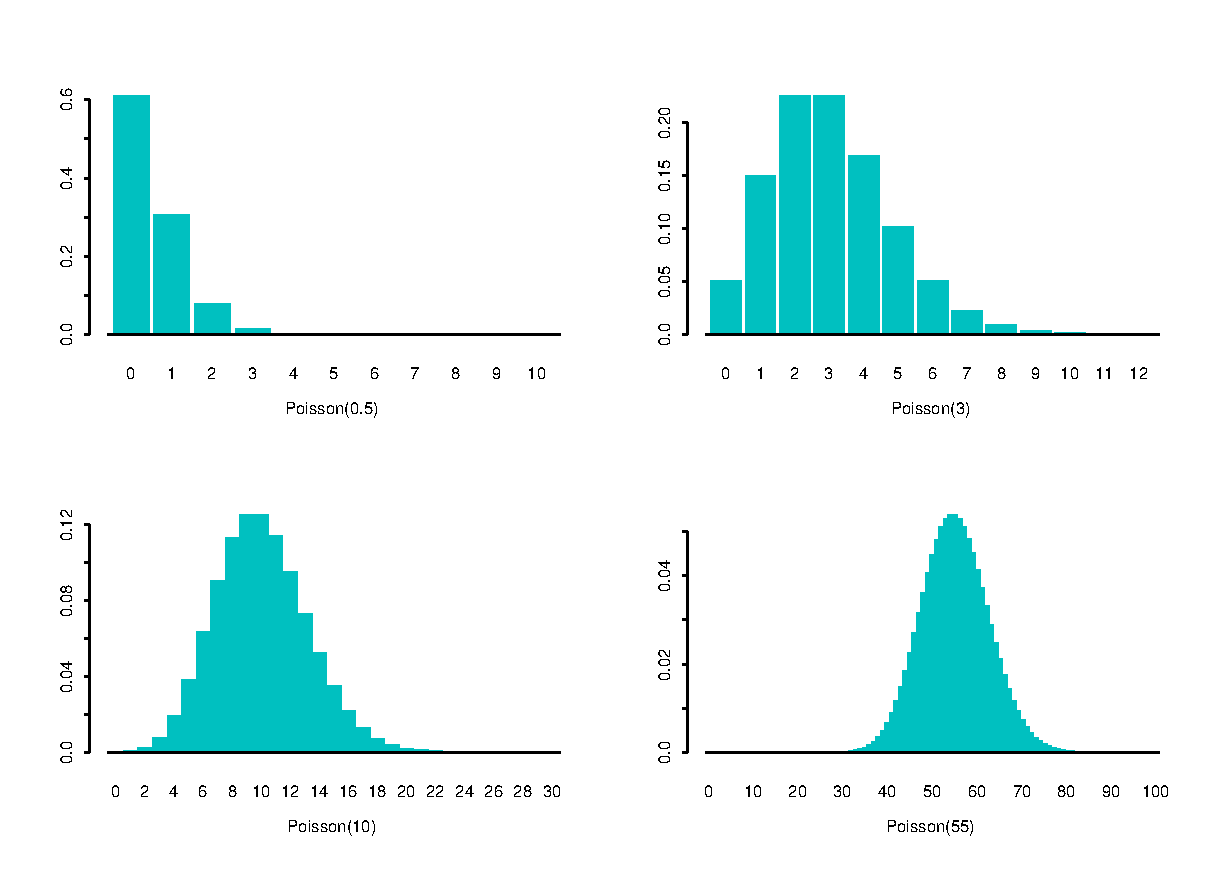
\includegraphics[width=0.75\textwidth]{img/distpois.pdf}
\end{figure}

\end{frame}%


\begin{frame}%
\frametitle{Poisson Distribution}

\begin{example}
The average number of newspapers sold by Alfred is 5 per minute\footnote{This number provides info on the intensity
at which a random phenomenon occurs.}. What is the probability that Alfred will sell at least 1 newspaper in a minute? \vspace{0.3cm}


To answer, let $X$ be the $\#$ of newspapers sold by Alfred in a minute. We have
$$
X \sim \text{Poisson}(\lambda)
$$
with $\lambda = 5$, so
\begin{eqnarray*}
P(X \geq 1) & = & 1- P(\{X=0\}) \\
& = & 1 - \exp^{-5} \frac{5^0}{0!} \\
%& = & 1-\exp^{-5} \\
& \approx & 1- 0.0067 \approx 99.33\%.
\end{eqnarray*}
How about $P(X \geq 2)$? Is it $P(X \geq 2) \geq P(X \geq 1)$ or not? Answer the question...
\end{example}
\end{frame}%



\begin{frame}%
\frametitle{Poisson Distribution}

\begin{example}
A telephone switchboard handles 300 calls, on the average, during one hour. The board
can make maximum 10 connections per minute. Use the Poisson
distribution to evaluate the probability that the board will be overtaxed during a given minute.

\vspace{0.4cm}

To answer, let us set  $\lambda = 300$ per hour, which is equivalent to 5 calls per minute. Noe let us define
$$
X = \text{\# of connections in a minute}
$$
and by assumption we have $X \sim \text{Poisson}(\lambda)$. Thus,
\bea
P[\text{overtaxed}] &=& P(\{X > 10\}) \nn \\
&=& 1 \quad - \underbrace{P(\{X \leq 10\})}_{\text{using $\lambda=5$,  minute base}} \nn \\
&\approx& 0.0137. \nn
\eea
\end{example}
\end{frame}


\begin{frame}%
%EndExpansion

\frametitle{Poisson Distribution (link to Binomial)}
Let us consider $X \sim B(x,n,p)$, \color{red} where $n$ is large, $p$ is small, and the product $np$ is appreciable\color{black}. Setting, $\lambda=np$, we
then have that, for the Binomial probability as in Eq.(\ref{Eq: Binom}), it is a good approximation to write:
$$
p(k) = P(\{X=k\}) \approx \frac{\lambda^k}{k!} e^{-\lambda}.
$$
To see this, remember that
$$
\lim_{n\rightarrow\infty} \left( 1- \frac{\lambda}{n} \right)^n = e^{-\lambda}.
$$
Then, let us consider that in our setting, we have $p=\lambda/n$. From the formula of the binomial probability mass function we have:
$$
p(0) = (1-p)^{n}=\left( 1- \frac{\lambda}{n} \right)^{n} \approx e^{-\lambda}, \quad \text{\ as \ \ } n\rightarrow\infty.
$$
\end{frame}%


\begin{frame}%
%EndExpansion

\frametitle{Poisson Distribution  (link to Binomial)}

Moreover, it is easily found that

\bea
\frac{p(k)}{p(k-1)} &=& \frac{np-(k-1)p}{k(1-p)} \approx \frac{\lambda}{k}, \quad \text{\ as \ \ } n\rightarrow\infty. \nn
\eea
Therefore, we have
\bea
p(1) &\approx& \frac{\lambda}{1!}p(0) \approx \lambda e^{-\lambda} \nn \\
p(2) &\approx& \frac{\lambda}{2!}p(1) \approx \frac{\lambda^2}{2} e^{-\lambda} \nn \\
\dotsm & \dotsm &  \dotsm  \nn \\
p(k) &\approx& \frac{\lambda}{k!}p(k-1) \approx \underbrace{\frac{\lambda^k}{k!} e^{-\lambda}}_{\text{\ see \ \ Eq. (\ref{Eq. Poisson})  }} \nn
\eea

thus, we remark that $p(k)$ can be approximated by the probability mass function of a Poisson---which is easier to implement.

\end{frame}%


\begin{frame}%
%EndExpansion

\frametitle{Poisson Distribution: example}
\begin{example}[two-fold use of Poisson]
Suppose a certain high-speed printer makes errors at random on printed paper\footnote{This exercise is related to Ex 2 of PS6. The calculation is similar but not identical: note the difference between the size of $p$ in this example and in the tutorial.}. Assuming that the Poisson
distribution with parameter $\lambda = 4$ is appropriate to model the number of errors per page (say, $X$), what is the probability that in a book containing 300 pages (produced by the printer) at least 7 will have no errors?

\vspace{0.3cm}
Let $X$ denote the number of errors per page, so that
$$
p(x) = \exp^{-4}\frac{4^x}{x!}, \quad \text{for} \quad x = 0,1,2,....
$$
The probability of any page to be error free is then
$$p(0) = \exp^{-4}\frac{4^0}{0!} = \exp^{-4} \approx 0.018.$$

\end{example}
\end{frame}%

\begin{frame}%
%EndExpansion

\frametitle{Poisson Distribution: example}
\begin{example}[cont'd]

Having no errors on a page is a success, and there are 300 independent pages. Hence, let us define
$$
Y = \text{the number of pages without any errors}.
$$

$Y$ is binomially distributed with parameters $n = 300$
and $p = 0.018$, namely
$$Y\sim B(n,p).$$

%\vspace{0.3cm}
But here we have
\begin{center}
$n$ large, $p$ small, and $n p = 5.4$
\end{center}
thus, we can compute $P(\{Y \geq 7\})$  using either the exact Binomial or its Poisson approximation. So
\begin{itemize}
\item using $B(300,0.018)$, we get: $P(\{Y \geq 7\}) \approx  0.297$ \\ \vspace{0.1cm}

\item using Poisson(5.4), we get $P(\{Y \geq 7\})  \approx  0.298.$
\end{itemize}

%The two outcomes differ at the 3rd digits after the comma.


\end{example}
\end{frame}%


\begin{frame}
\frametitle{The Hypergeometric Distribution}

\begin{definition}
Let us consider a random experiment consisting of a series of $n$ trials,
having the following properties

\begin{stepenumerate}
\item Only two mutually exclusive outcomes are possible in each trials:
success (S) and failure (F)

\item The population has $N$ elements in which $k$ are looked upon as
S and the other $N-k$ are looked upon as F

\item Sampling from the population is done \textbf{without} replacement (so
that the trials are not independent).
\end{stepenumerate}
The random variable
$$
X= \text{number of successes in $n$ such
trials}
$$
has an hypergeometric distribution and ....
\end{definition}

%TCIMACRO{\TeXButton{EndFrame}{\end{frame}}}%
%BeginExpansion
\end{frame}%
%EndExpansion

%TCIMACRO{\TeXButton{BeginFrame}{\begin{frame}}}%
%BeginExpansion
\begin{frame}%
%EndExpansion

\frametitle{The Hypergeometric Distribution}

\begin{definition}[cont'd]
... the probability that $X=x$ is
\begin{equation*}
\Pr (\left\{ X=x\right\}) =\frac{\left(
\begin{array}{c}
k \\
x%
\end{array}%
\right) \left(
\begin{array}{c}
N-k \\
n-x%
\end{array}%
\right) }{\left(
\begin{array}{c}
N \\
n%
\end{array}%
\right) }.
\end{equation*}
\end{definition}

Moreover,
\begin{eqnarray*}
E\left[ X\right] &=&\frac{nk}{N} \\
Var\left( X\right) &=&\frac{nk\left( N-k\right) \left( N-n\right) }{%
N^{2}\left( N-1\right) }
\end{eqnarray*}

%TCIMACRO{\TeXButton{EndFrame}{\end{frame}}}%
%BeginExpansion
\end{frame}%
%EndExpansion

%TCIMACRO{\TeXButton{BeginFrame}{\begin{frame}}}%
%BeginExpansion
\begin{frame}%
%EndExpansion

\frametitle{Hypergeometric Distribution Example}

\begin{example}[Psychological experiment]
A group of 8 students includes 5 women and 3 men: 3 students are randomly chosen to participate in a psychological
experiment. What is the probability that \emph{exactly} 2 women will be included
in the sample?%
%TCIMACRO{%
%\FRAME{ftbpF}{2.1966in}{2.207in}{0pt}{}{}{urnpic.gif}{%
%\special{language "Scientific Word";type "GRAPHIC";maintain-aspect-ratio TRUE;display "USEDEF";valid_file "F";width 2.1966in;height 2.207in;depth 0pt;original-width 6.9168in;original-height 6.9479in;cropleft "0";croptop "1";cropright "1";cropbottom "0";filename '../URNpic.GIF';file-properties "XNPEU";}}}%
%BeginExpansion
\begin{figure}[ptb]\centering
%\includegraphics[natheight=6.9479in, natwidth=6.9168in, height=2.207in, width=2.1966in]
%{//ad.monash.edu/home/User063/scipione/Documents/CF2015/teaching/ETC2520/NEW_ETC25250/lecture6_2015/graphics/img/URNpic__2.pdf}%
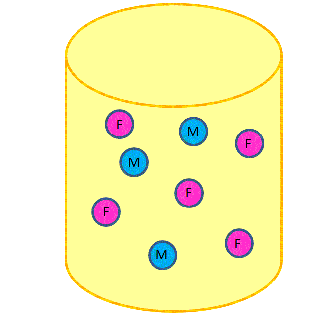
\includegraphics[width=0.4\textwidth]{img/URNpic_2.pdf}
\end{figure}%
%EndExpansion
\end{example}

%TCIMACRO{\TeXButton{EndFrame}{\end{frame}}}%
%BeginExpansion
\end{frame}%
%EndExpansion

%TCIMACRO{\TeXButton{BeginFrame}{\begin{frame}}}%
%BeginExpansion
\begin{frame}%
%EndExpansion

\frametitle{Hypergeometric Distribution Example}

\begin{example}[cont'd]
Consider each of the three participants being selected as a separate
trial $\Rightarrow $ there are $n=3$ trials. Consider a woman being selected in a trial as a `success'
\\
Then here $N=8$, $k=5$, $n=3$, and $x=2$, so that%
\begin{eqnarray*}
\Pr (\left\{ X=2\right\})  &=&\frac{\left(
\begin{array}{c}
5 \\
2%
\end{array}%
\right) \left(
\begin{array}{c}
8-5 \\
3-2%
\end{array}%
\right) }{\left(
\begin{array}{c}
8 \\
3%
\end{array}%
\right) } \\
&& \\
&=&\frac{\frac{5!}{2!3!}\frac{3!}{1!2!}}{\frac{8!}{5!3!}} \\
&& \\
&=&0.53571
\end{eqnarray*}
\end{example}

%TCIMACRO{\TeXButton{EndFrame}{\end{frame}}}%
%BeginExpansion
\end{frame}%
%EndExpansion

%TCIMACRO{\TeXButton{BeginFrame}{\begin{frame}}}%
%BeginExpansion
\begin{frame}%
%EndExpansion

\frametitle{The Negative Binomial Distribution}

Let us consider a random experiment consisting of a series of trials, having
the following properties \vspace{0.5cm}

\begin{stepenumerate}
\item Only two mutually exclusive outcomes are possible in each trial:
`success' (S) and `failure' (F)
\vspace{0.25cm}
\item The outcomes in the series of trials constitute \emph{independent
events}
\vspace{0.25cm}
\item The probability of success $p$ in each trial is \emph{constant }from
trial to trial
\end{stepenumerate}
\vspace{0.5cm}
What is the probability of having exactly $y$ F's before the $r^{th}$
S? \\ \vspace{0.25cm}

Equivalently: What is the probability that in a sequence of $y+r$ (Bernoulli) trials the last trial yields the
$r^{th}$ S?


%TCIMACRO{\TeXButton{EndFrame}{\end{frame}}}%
%BeginExpansion
\end{frame}%
%EndExpansion

%TCIMACRO{\TeXButton{BeginFrame}{\begin{frame}}}%
%BeginExpansion
\begin{frame}%
%EndExpansion

\frametitle{The Negative Binomial Distribution}

\begin{definition}
Let
$$X= \text{the total number of trials required until a total of $r$ successes is accumulated}.$$
Then $X$ is said to be a Negative Binomial random variable and its probability mass function
$\Pr (\left\{ X=n\right\})$ equals the probability of $r-1$ `successes' in the first $n-1$ trials, times the probability of a `success' on
the last trial. These probabilities are given by%
\begin{equation*}
\Pr (\left\{ X=n\right\}) =\left(
\begin{array}{c}
n-1 \\
r-1%
\end{array}%
\right) p^{r}\left( 1-p\right) ^{n-r}\quad \text{ for }n=r,r+1,...
\end{equation*}
\end{definition}

The mean and variance for $X$ are, respectively,%
\begin{eqnarray*}
E\left[ X\right] &=&\frac{r}{p} \\
Var\left( X\right) &=&\frac{r\left( 1-p\right) }{p^{2}}
\end{eqnarray*}

%TCIMACRO{\TeXButton{EndFrame}{\end{frame}}}%
%BeginExpansion
\end{frame}%
%EndExpansion

%TCIMACRO{\TeXButton{BeginFrame}{\begin{frame}}}%
%BeginExpansion
\begin{frame}%
%EndExpansion

\frametitle{Negative Binomial Distribution Example}

\begin{example}[marketing research]
\begin{stepitemize}

\item A marketing researcher wants to find 5 people to join her focus group

\item Let $p$ denote the probability that a randomly selected individual
agrees to participate in the focus group

\item If $p=0.2$, what is the probability that the researcher must ask 15
individuals before 5 are found who agree to participate?

%\item That is, what is the probability that 10 people will decline the
%request to participate before a 5$^{th}$ person agrees?

\item In this case, $p=0.2$, $r=5$, $n=15$:  we are looking for $\Pr (\left\{
X=15\right\}).$ By the negative binomial formula we have

\begin{eqnarray*}
\Pr (\left\{ X=15\right\}) &=&\left(
\begin{array}{c}
14 \\
4%
\end{array}%
\right) \left( 0.2\right) ^{5}\left( 0.8\right) ^{10} \\
&=&0.034
\end{eqnarray*}
\end{stepitemize}
\end{example}
%TCIMACRO{\TeXButton{EndFrame}{\end{frame}}}%
%BeginExpansion
\end{frame}%
%EndExpansion

%TCIMACRO{\TeXButton{BeginFrame}{\begin{frame}}}%
%BeginExpansion
\begin{frame}%
%EndExpansion

\frametitle{The Geometric Distribution}

\begin{definition}[a special case]

When $r=1$, the negative binomial distribution is equivalent to the
\textbf{Geometric distribution} --- see Example in slide 13. \\
\vspace{0.5cm}
In this case, probabilities are given by%
\begin{equation*}
\Pr (\left\{ X=n\right\}) =p\left( 1-p\right) ^{n-1}\text{, for }n=1,2,...
\end{equation*}
\end{definition}

The corresponding mean and variance for $X$ are, respectively,%
\begin{eqnarray*}
E\left[ X\right] &=&\frac{ 1 }{p} \\
Var\left( X\right) &=&\frac{\left( 1-p\right) }{p^{2}}
\end{eqnarray*}


\end{frame}

\begin{frame}

\frametitle{The Geometric Distribution}
\begin{small}

\begin{example}[failure of a machine]
Items are produced by a machine having a 3\% defective rate.
\begin{itemize}
\item What is the probability that the first defective occurs in the fifth item inspected? \\
\bea
P(\{X	=	5\})	&=&	P (\text{first	4	non-defective}) P (\text{5th defective}) \nn \\
&=& (0.97)^4(0.03) \approx 0.026 \nn
\eea
\item What is the probability that the first defective occurs in the first five inspections?
\bea
P(\{X	\leq 5	\}) = P(\{X	< 6	\})	&=&	 P (\{X=1\})+ ... + P(\{X=5\}) \nn \\
&=& 1- P(\text{first 5 non-defective}) = 0.1412.  \nn %\\
%&=& 1- (0.97)^5 \approx 0.1412 \nn
\eea
\end{itemize}
\end{example}

More generally, for a geometric random variable we have:
$$
P(\{X \geq k \}) = (1-p)^{k-1}.
$$
Thus, in the example we have $P( \{X	\geq 6	\}) = (1-0.03)^{6-1}\approx 0.8587$
\bea
P(\{X	\leq 5	\}) = 1-P( \{X	\geq 6	\}) \approx 1- 0.8587 \approx 0.1412. \nn
\eea

\end{small}



\end{frame}



\end{document}
